% 0622 v3.0 plan
% -[x] 将 word 批注和修改内容整理到 tex 中
% -[x] 确定修改要点,批注和obsidian记录

% 0623 v3.0 plan 具体修改计划
% !!!!!! 先改方法、后改案例、最后改介绍和其他
% -[ ] 题目 点明我们的普适性、自动化?
% -[ ] 摘要 中间段重写;点明普适性、自动化
% -[ ] introduction 
%      -[ ] 不放案例;
%      -[ ] 增加重构灵活性的文献;
%      -[ ] 有向图的文献;
%      -[ ] 点明普适性、自动化
% -[ ] methodology 
%      -[x] main 图重画,只保留文字;
%      -[x] 有向图模型,说清三层关系,更规矩地写建模过程;
%      -[x] 优化目标和约束;
%      -[ ] 最短路径,逐句逐字去捋顺;
%      -[ ] 贪心算法,结合流程图说明算法过程,把二分法融进去;
%      -[ ] 增加隔离的处理,如约束、算法的改动
% -[ ] case study 
%      -[ ] 考虑新结构(MAC=4,想不到就算了,仍用ef结构);
%      -[ ] results 直接给出结果,略去计算细节;
%      -[ ] discussion 说明eta的合理性;
%      -[ ] 什么样的结构能获得更大的MAC(易隔离性和输出性能的冲突)(想不出来就算了);
%      -[ ] 电池隔离场景下的MAC变化(比较不同结构)

% keep in mind
% 1. 用最简洁、读者最能接受的话说明清楚自己想表达的内容

% mark
% 统一为 directed graph model
% 统一用 electrical load 而非 electrical appliance (泛指家电)

% magic
% 你将扮演一位英文学术写作经验丰富的大学老师,指导一位非英文母语的学生完成并改进他的论文。 你的目标是帮助他写出一篇流畅、清晰、易读、符合规范的英文学术论文。 他会向你用中文说明自己想表达的内容,有时还会给你一些不完整的英文句子让你补充完整。你不应该逐字翻译他的内容,你需要和他经过多次的沟通,以确定最好的表达。 注意,你们交流的内容可能包含latex语法,你需要理解并使用;当你形成完整的句子或段落时,你要将这些句子或段落放在```\n 和\n ```之间,即 ```\n some sentence\n ```,其中每写完一句话都要换行。

\documentclass{article}
\usepackage{graphicx}
\usepackage{subcaption}
\usepackage{enumerate}
\usepackage{amsmath}
\DeclareMathOperator{\diag}{diag}
\usepackage{multirow}
\usepackage{booktabs}
\usepackage{bm}
\usepackage[ruled,linesnumbered]{algorithm2e}
\setcounter{MaxMatrixCols}{20}
\usepackage{tikz}
\usetikzlibrary{arrows.meta, calc, fit, positioning, quotes, graphs, shapes.geometric}
\def\T{\mathrm{T}}


\title{Maximum Allowable Current Determination of Arbitrary Reconfigurable Battery Systems By Using a Directed Graph Model Combined with Greedy Algorithm}
\author{3057761608 }

\begin{document}

\maketitle

\begin{abstract} % #TODO: rewrite
    Reconfigurable Battery Systems (RBSs) offer a promising alternative to traditional battery systems owing to their flexible and dynamic changeable topologic structure subjected to battery cell charging and discharging strategies. 
    During the operation of the RBS, Maximum Allowable Current (MAC) is a critical indicator to guide the reconfiguring control of the system in terms of safety and reliability. 
    In this paper, the MAC of the RBS is calculated by using a greedy algorithm based on the directed graph model of the RBS. % 这句话展开讲, Greedy algorithm方法被用于…/与…方法相结合,实现了对任意RBS结构的MAC提取,
    % The greedy algorithm method has been used to solve a model based on topology structure, achieving MAC estimation for any RBS structure.
    The effectiveness of this method is validated on a more complex RBS structure based on two proposed structure. 
    This proposed Greedy-based method paves the way for more flexible design and more complex application scenarios, such as battery cell isolation, for RBS.

    keywords:  Reconfigurable Battery System, Maximum Allowable Current, Greedy Algorithm
\end{abstract}

\section{Introduction}
% 不放案例
% 重构灵活性的文献
% 有向图的文献

Battery Energy Storage Systems (BESSs) are widely used to store and release high-quality electrical energy in various applications, such as smart grids and wind power plants \cite{desiqueiraControlStrategySmooth2021,karandehTwoStageAlgorithmOptimal2019,yangBatteryEnergyStorage2018,choCommercialResearchBattery2015}.
Typically, a BESS consists of numerous battery cells that are interconnected by series-parallel circuitry to provide the required capacity storage.
The traditional BESS, in which the batteries are connected in a fixed topology, has a significant weakness on its worst battery, caused by the so-called cask effect.
Furthermore, if this worst battery is failed during the operation process, it will exacerbate the degradation of the other batteries with a high possibility, and arouse reliability and even safety issues \cite{yangUnbalancedDischargingAging2016,fengPropagationMechanismsDiagnosis2019}.


Reconfigurable Battery System (RBS), which can dynamically switch to different circuit topology configurations as required, is expected to solve the above problem\cite{hanNextGenerationBatteryManagement2020a}.
The ability of switching circuit helps to isolate unhealthy batteries, and thereby improve the safety and reliability of the battery system.
Fig. \ref{fig:arch} shows two popular typologies of the RBSs developed by Lawson\cite{lawsonSoftwareConfigurableBattery2012} and Visairo \cite{visairoReconfigurableBatteryPack2008} respectively. 
Taking the RBS shown in Fig. \ref{fig:arch-e} as example, the batteries in the RBS can be connected not only in series when the switches $S_1$, $S_5$, $S_6$, $S_7$, $S_8$, $S_9$, and $S_{13}$ are closed, but also in parallel when $S_1$, $S_2$, $S_3$, $S_4$, $S_5$, $S_9$, $S_{10}$, $S_{11}$, $S_{12}$, and $S_{13}$ are closed.
Furthermore, when an unhealthy battery, for instance the orange one in Fig. \ref{fig:arch-f}, exits in the RBS, it can be isolated by closing its three adjacent switches (i.e. $S_5$, $S_7$ and $S_8$) and opening the switch below that battery (i.e. $S_6$) to ensure the system still remains a reliable working mode.
% 补充一句话总结,visairo的网络与固定串并联结构相比具有哪些优点,更适合使用在什么场合

\begin{figure}[htbp]
    \centering
    \begin{subfigure}[b]{0.2\textwidth}
        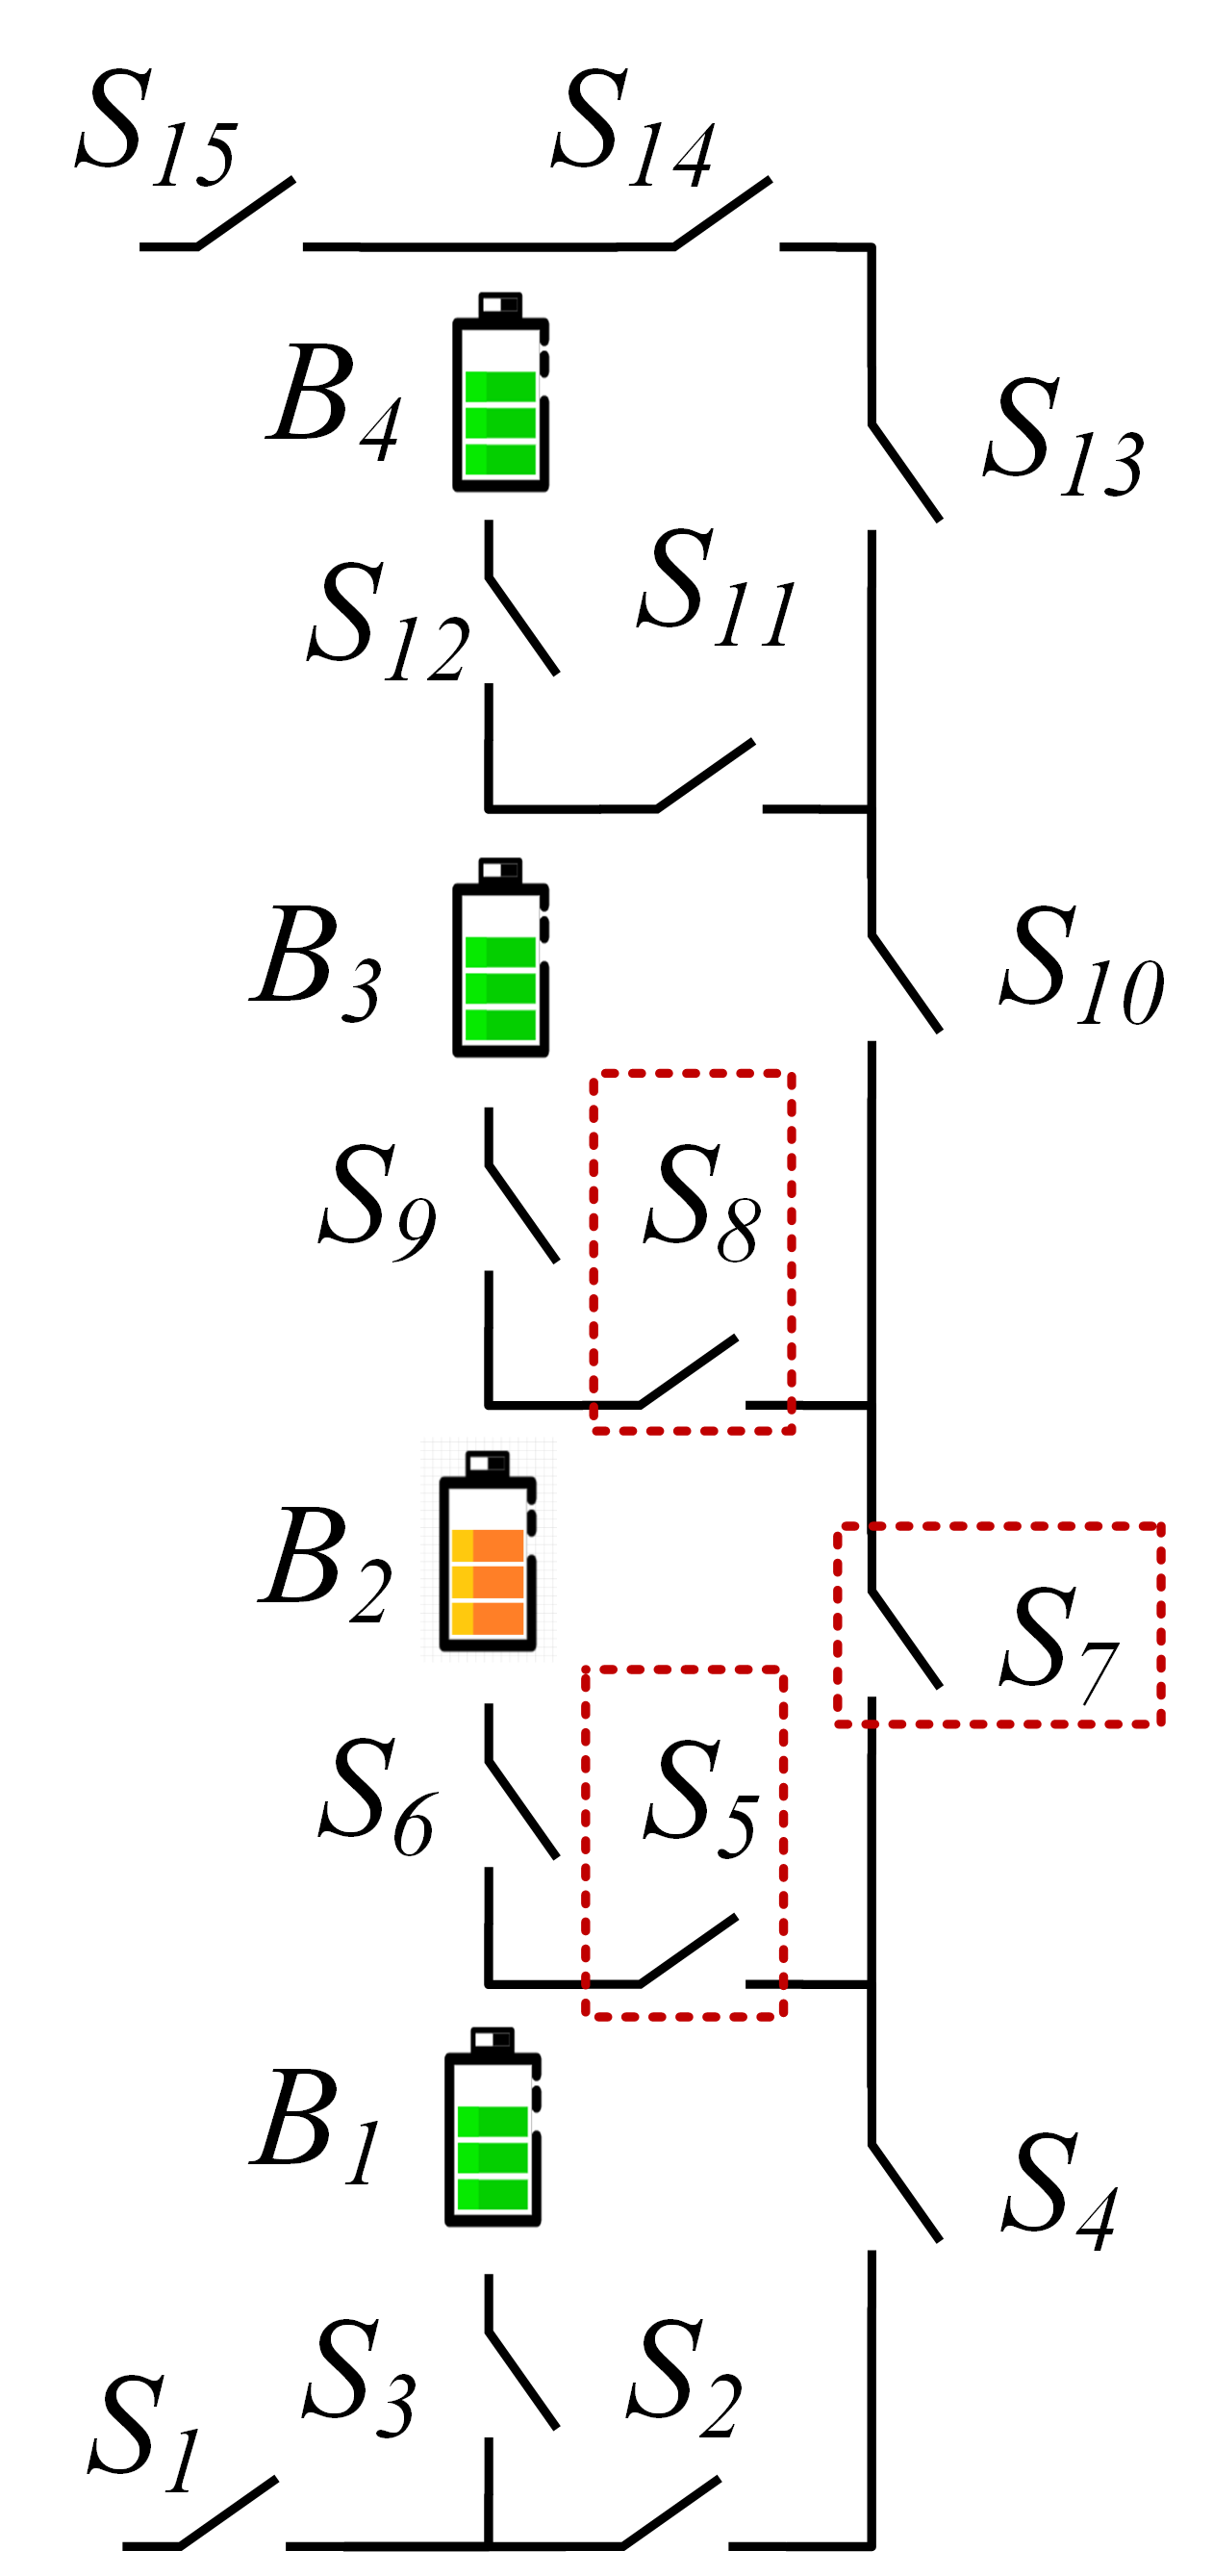
\includegraphics[width=\textwidth]{../attachments/arch-e.png}
        \caption{}
        \label{fig:arch-f}
    \end{subfigure}
    \hspace{0.05\textwidth}
    \begin{subfigure}[b]{0.45\textwidth}
        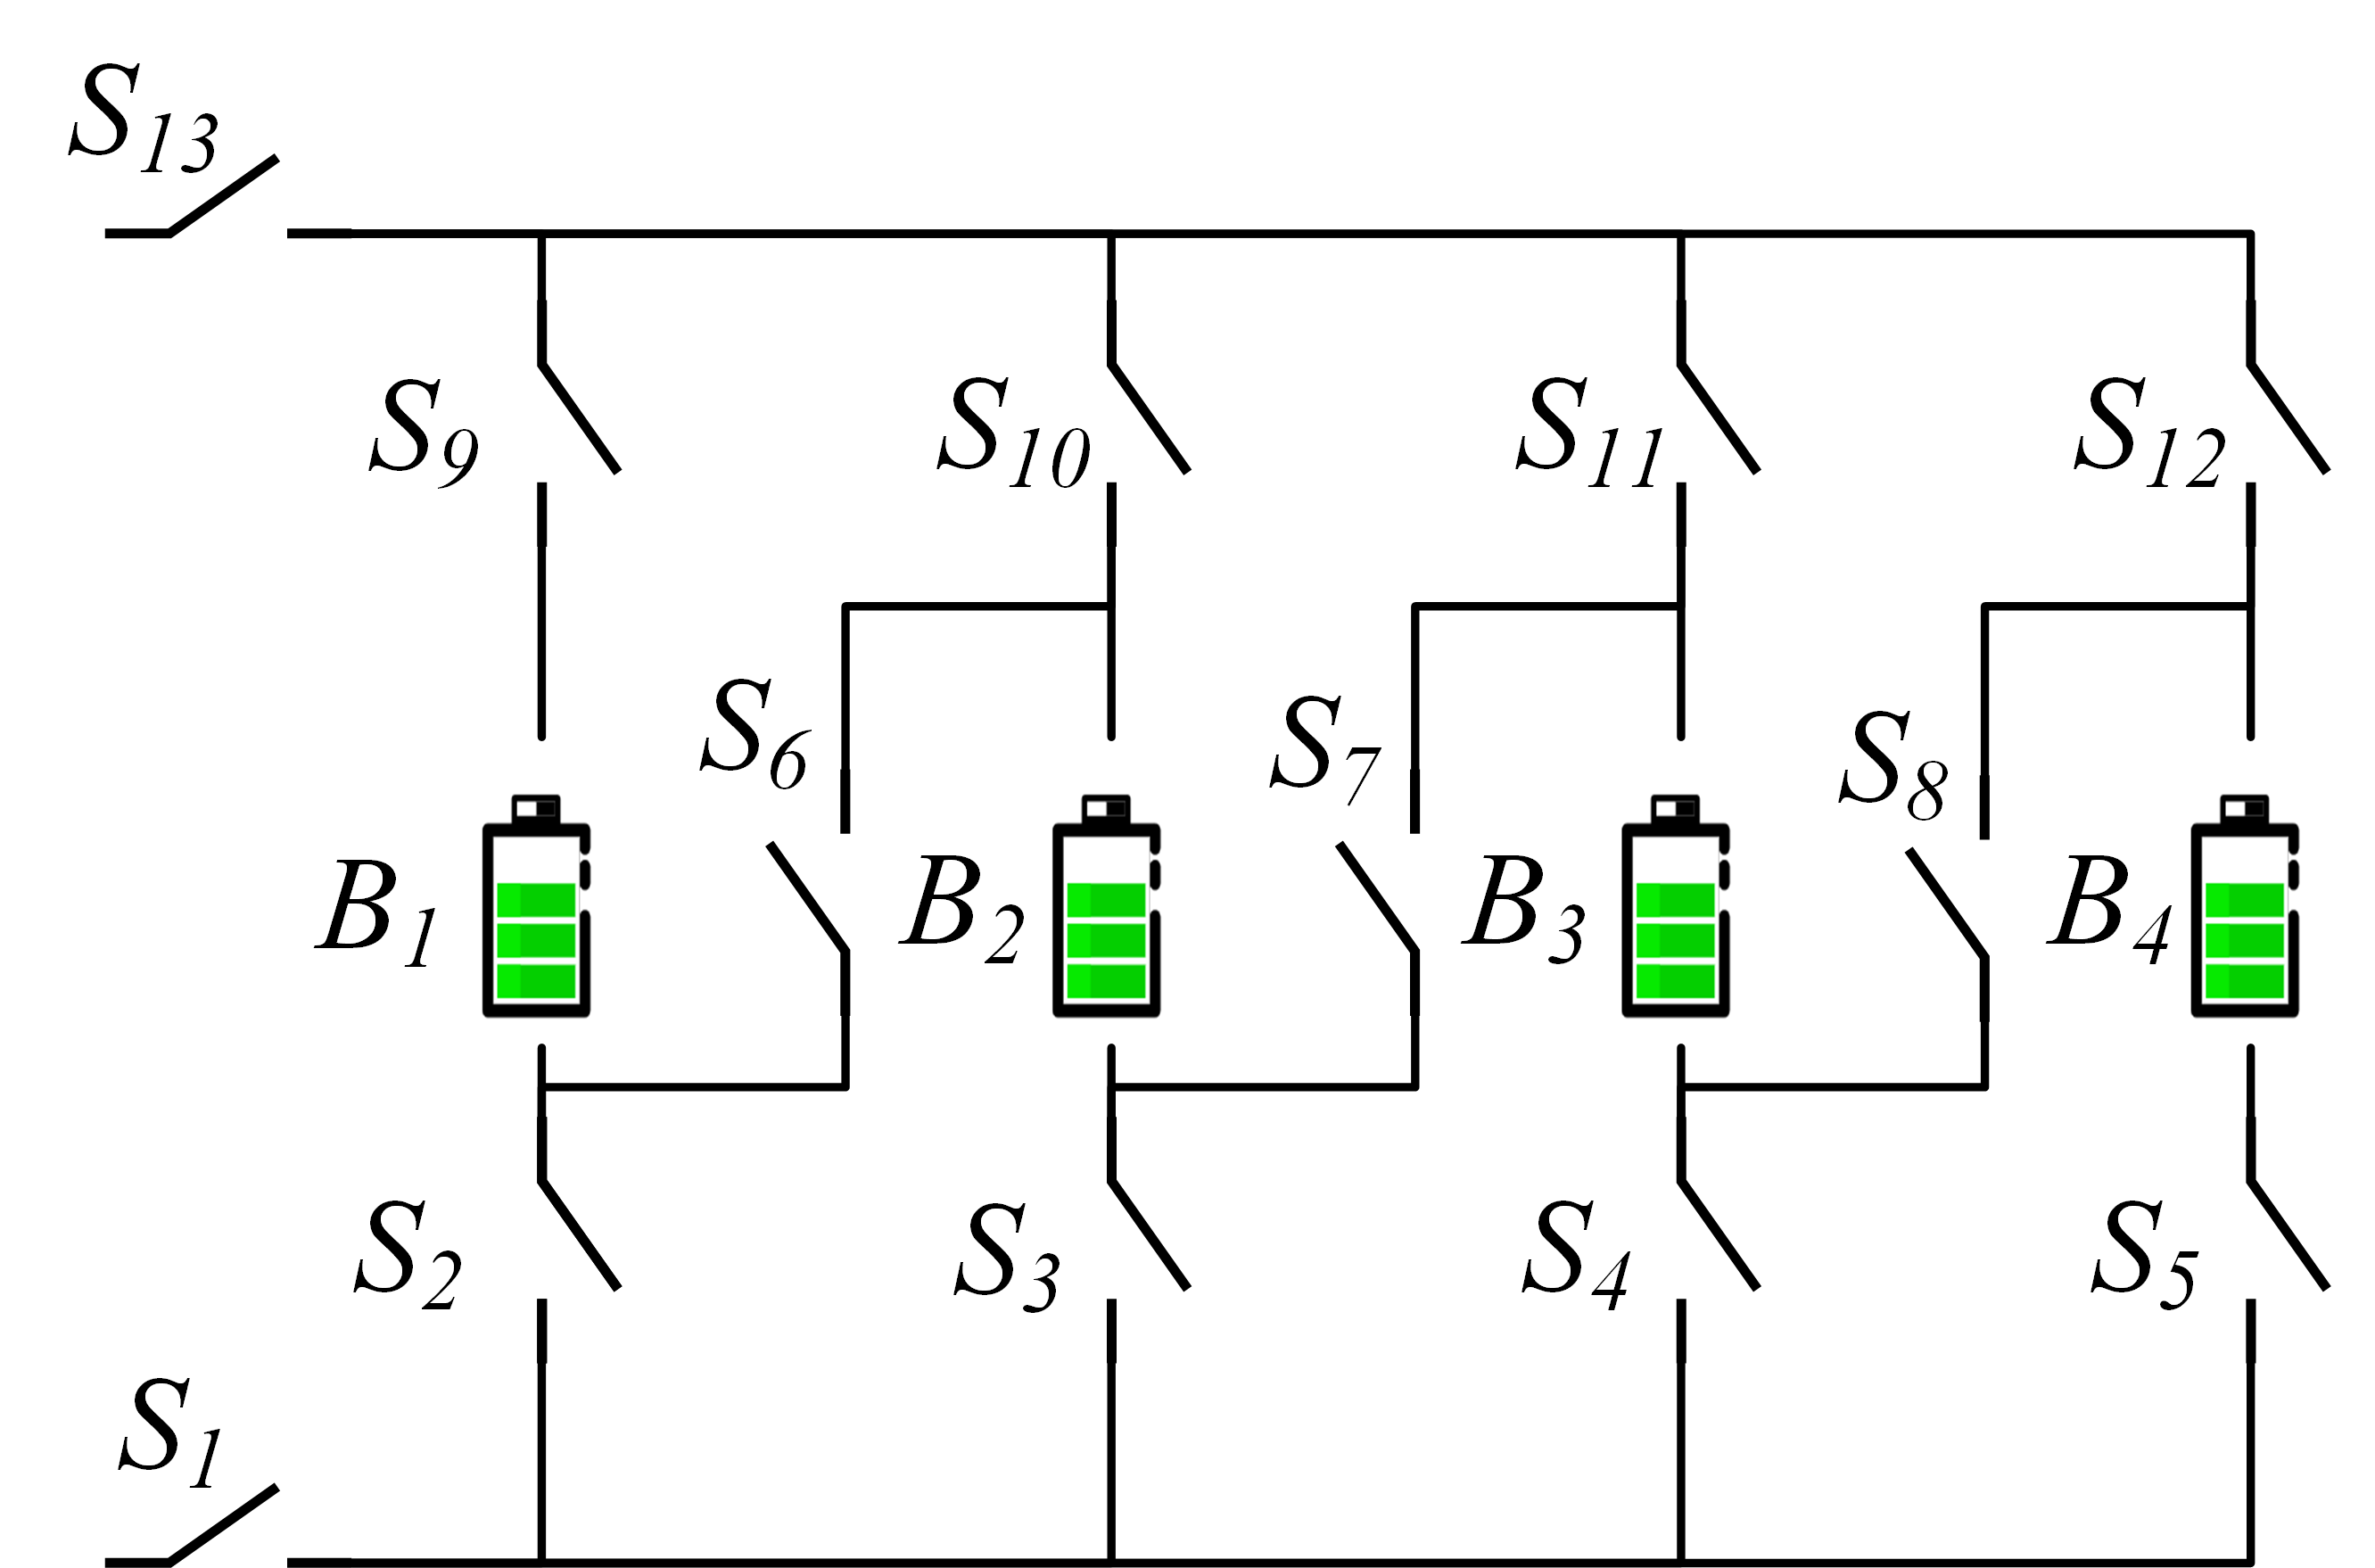
\includegraphics[width=\textwidth]{../attachments/arch-f.png}
        \caption{}
        \label{fig:arch-e}
    \end{subfigure}
    \caption{The RBS structure proposed by (a)Lawson\cite{lawsonSoftwareConfigurableBattery2012}, (b)Visairo\cite{visairoReconfigurableBatteryPack2008}.}
    \label{fig:arch}
\end{figure}

The complex connecting structure between batteries and switches enables the flexibility of the RBS, but on the other hand brings the challenges in desgin and control cost as well.
All switches of the RBS need to be controlled to output currents and powers that match the external load in read-time while avoiding batteries short-circuit.
The Maximum Allowable Current (MAC) of the RBS system is defined as the maximum current that is allowed for each individual battery of the system, and is a critical indictor to be evaluate the RBS output current to the electronic appliances.% 这里缺少过渡,MAC和设计与控制成本有什么关系?
It helps the designer to assess whether the RBS meets the output current requirements, and contributes to the formulation of appropriate and safe management stragegies for the battery management system (BMS). 
Despite its importance, there is currently no way to automatically evaluate MAC for RBSs. 
Especially when one (or more) stochastic battery is isolated, it is not possible to simultaneously determine the MAC of the rest of the RBS to assist the BMS to provide a timely adjustment of the control strategy. 
Under such circumstance, a universal and effective method for calculating the MAC of the RBS is urgently needed for the practical application of RBSs. 
To achieve this, a directed graph model that builds the relationship between RBS circuit topology and internal resistance and voltage of its batteries are established. 
Then, a greedy algorithm is employed to search the available circuit of the RBS for reaching the MAC.
% 以上两句话争取合并成一句话,提出的方法应该紧扣标题(即与标题的方法一致)
With this proposed method, the MAC of RBSs with arbitrary structures can be calculated effectively, including application scenarios with isolated battery cells.


The remainder of this paper is organized as follows: 
Section II presents the framework and details of the proposed topologic model and the greedy algorithm. 
In Section III, a case study of using the proposed model and algorithm to enumerate the MAC of a new and complex structure is demonstrated. 
The calculation results and scenarios such as battery cells isolation also are discussed. 
Finally, the concluding remarks are drawn in Section IV.


\section{Methodology}

The central principle of this method is to make the batteries in RBS connected in series as much as possible, thereby maximizing the output current of the RBS.
To universally and automatically achieve this, the overall process is divided into four steps, as shown in Fig. \ref{fig:main}.
Firstly, a directed graph model is established for subsequent computing, which not only contains the connected relationships between batteries and switches, but also retains the performance parameters of the batteries.
Subsequently, based on the equivalent circuit, the MAC problem is transformed into specific objective functions and constraints.
Then, the shortest paths (SPs, where additional batteries and switches on the path are penalized as distance) for the batteries are obtained using the Dijkstra algorithm to guide the batteries in the RBS connect in series.
Finally, a greedy algorithm is employed to organize the switches, allowing the batteries to connect via their SPs while satisfying the constraints, resulting in the MAC of the RBS.

\begin{figure}[htbp]
    \centering
    \begin{subfigure}[b]{0.8\textwidth}
        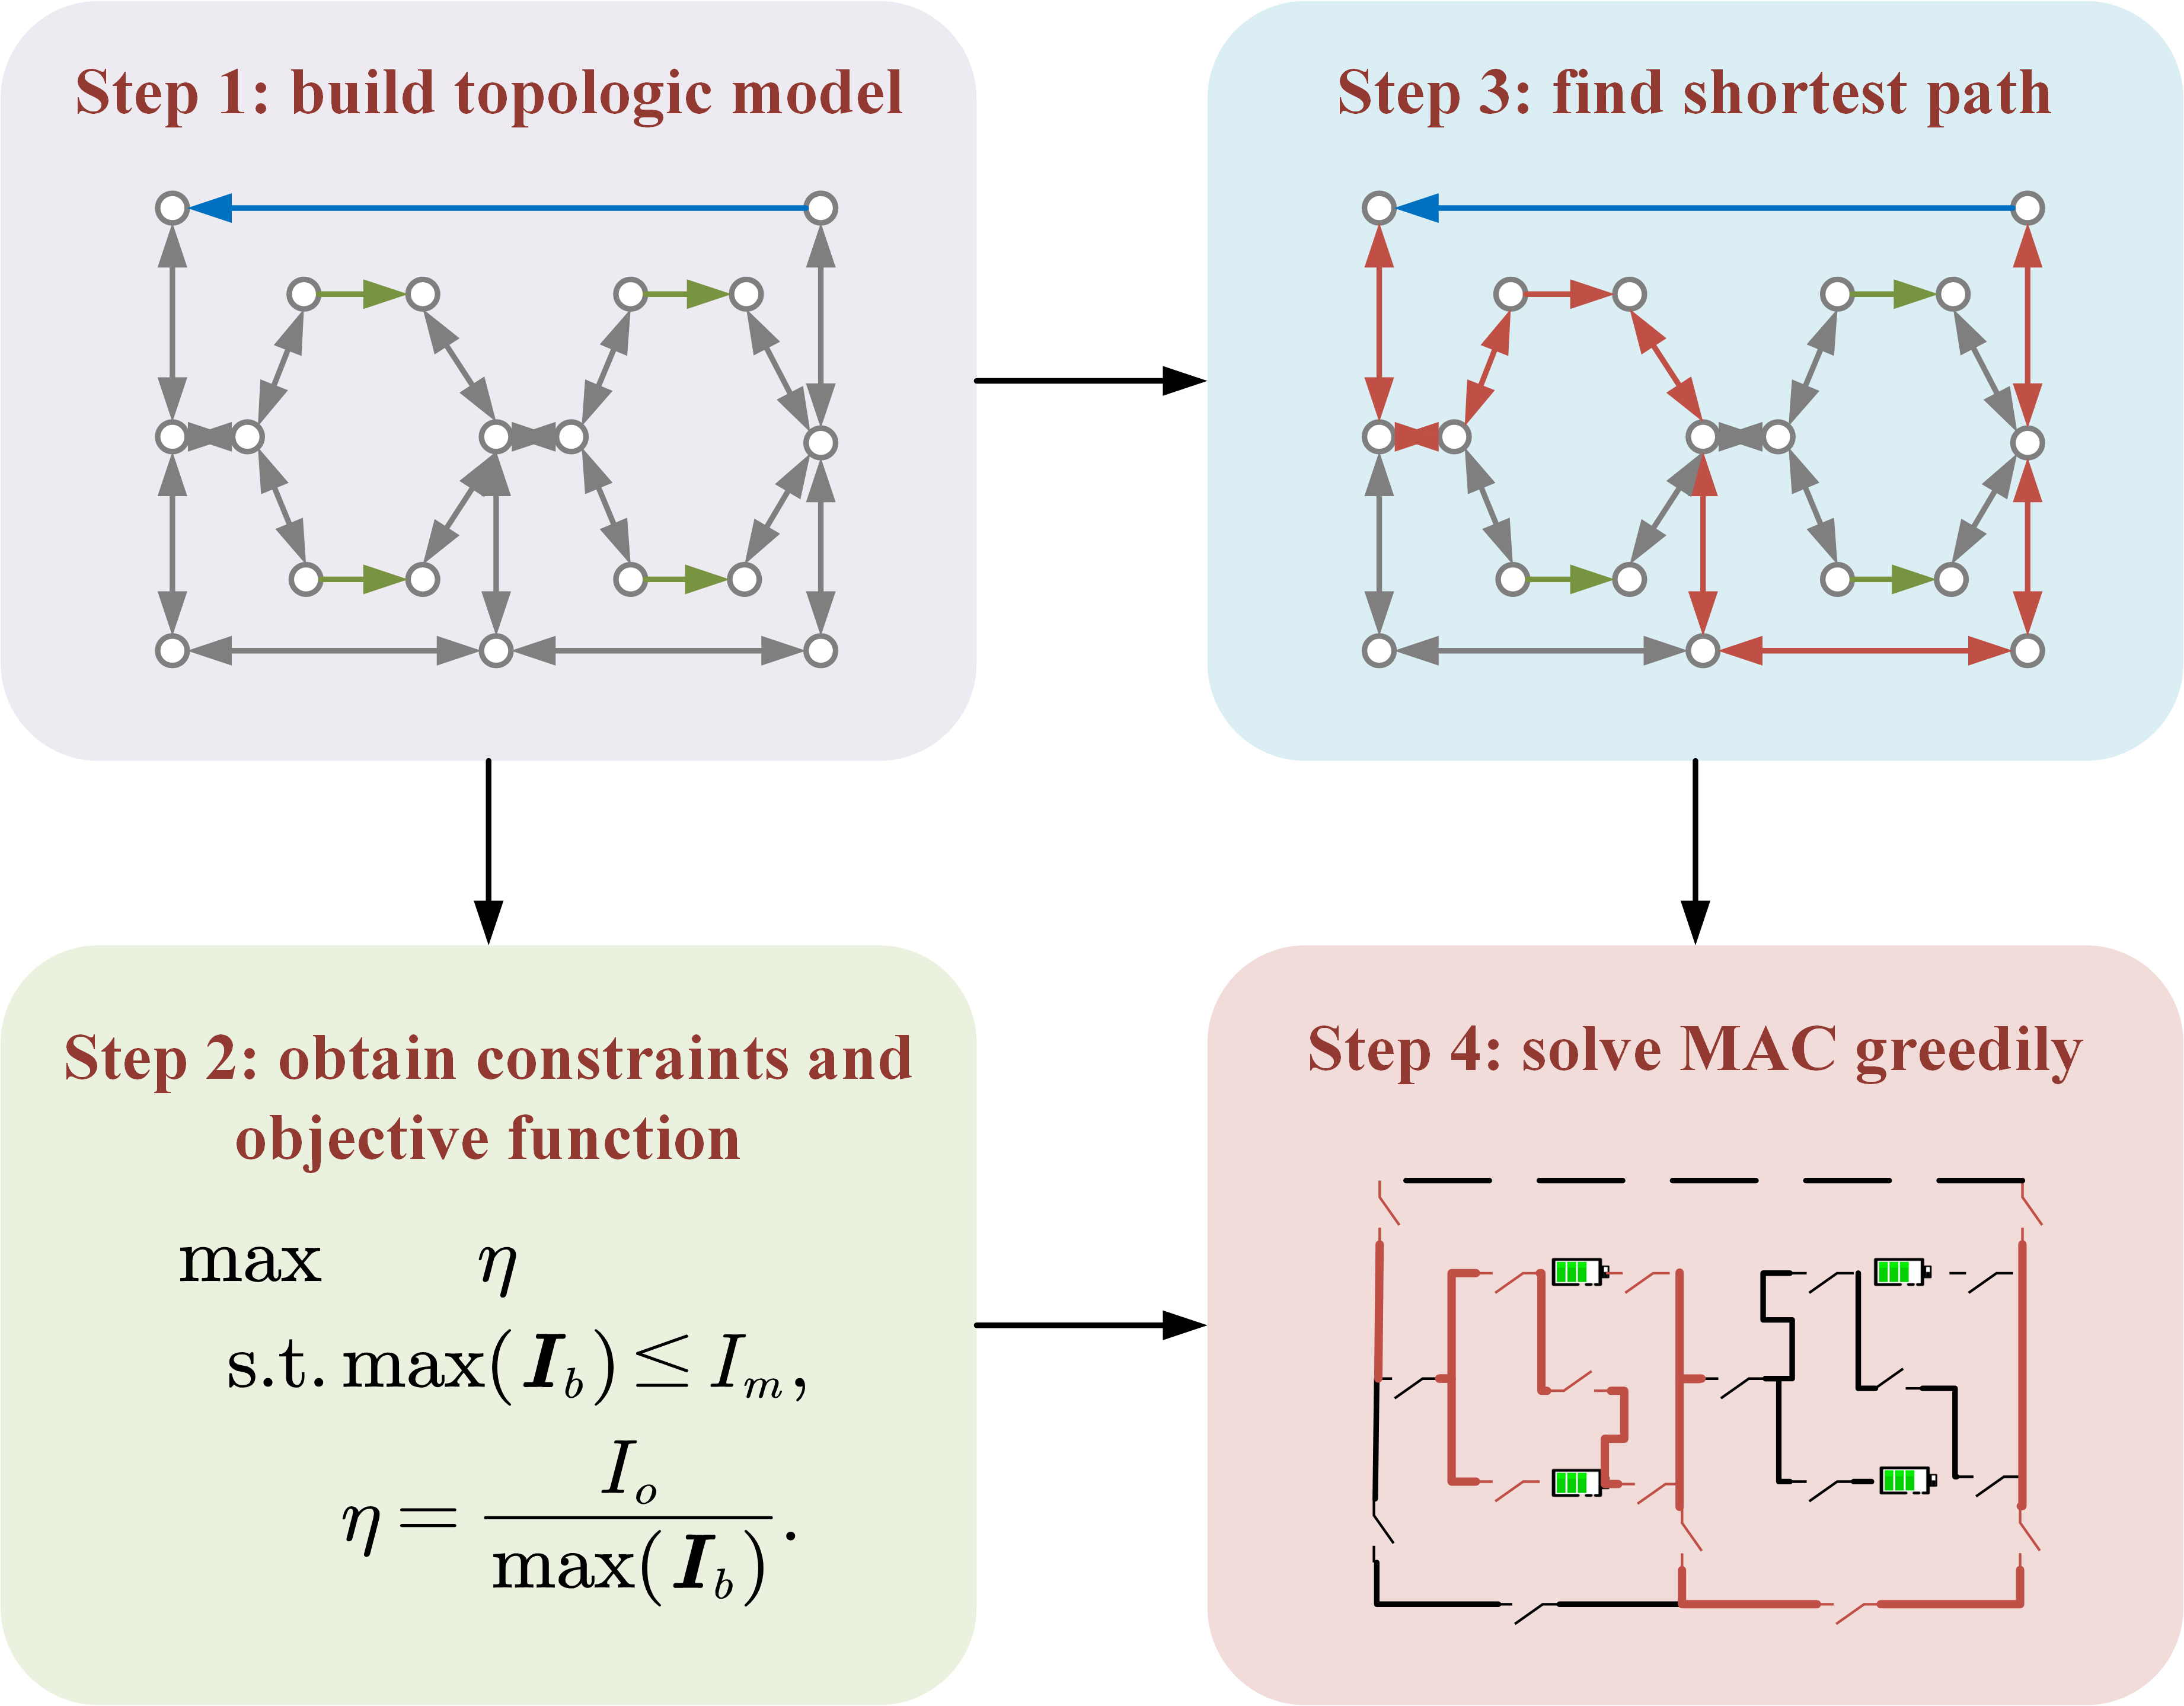
\includegraphics[width=\textwidth]{../attachments/main.png}
        \caption{}
        \label{fig:main}
    \end{subfigure}
    \caption{ 
        Diagram of this method, which contains four main steps.
    }
\end{figure}

\subsection{Directed graph Model}

\begin{figure}[htbp]
    \centering
    \begin{subfigure}[b]{0.31\textwidth}
        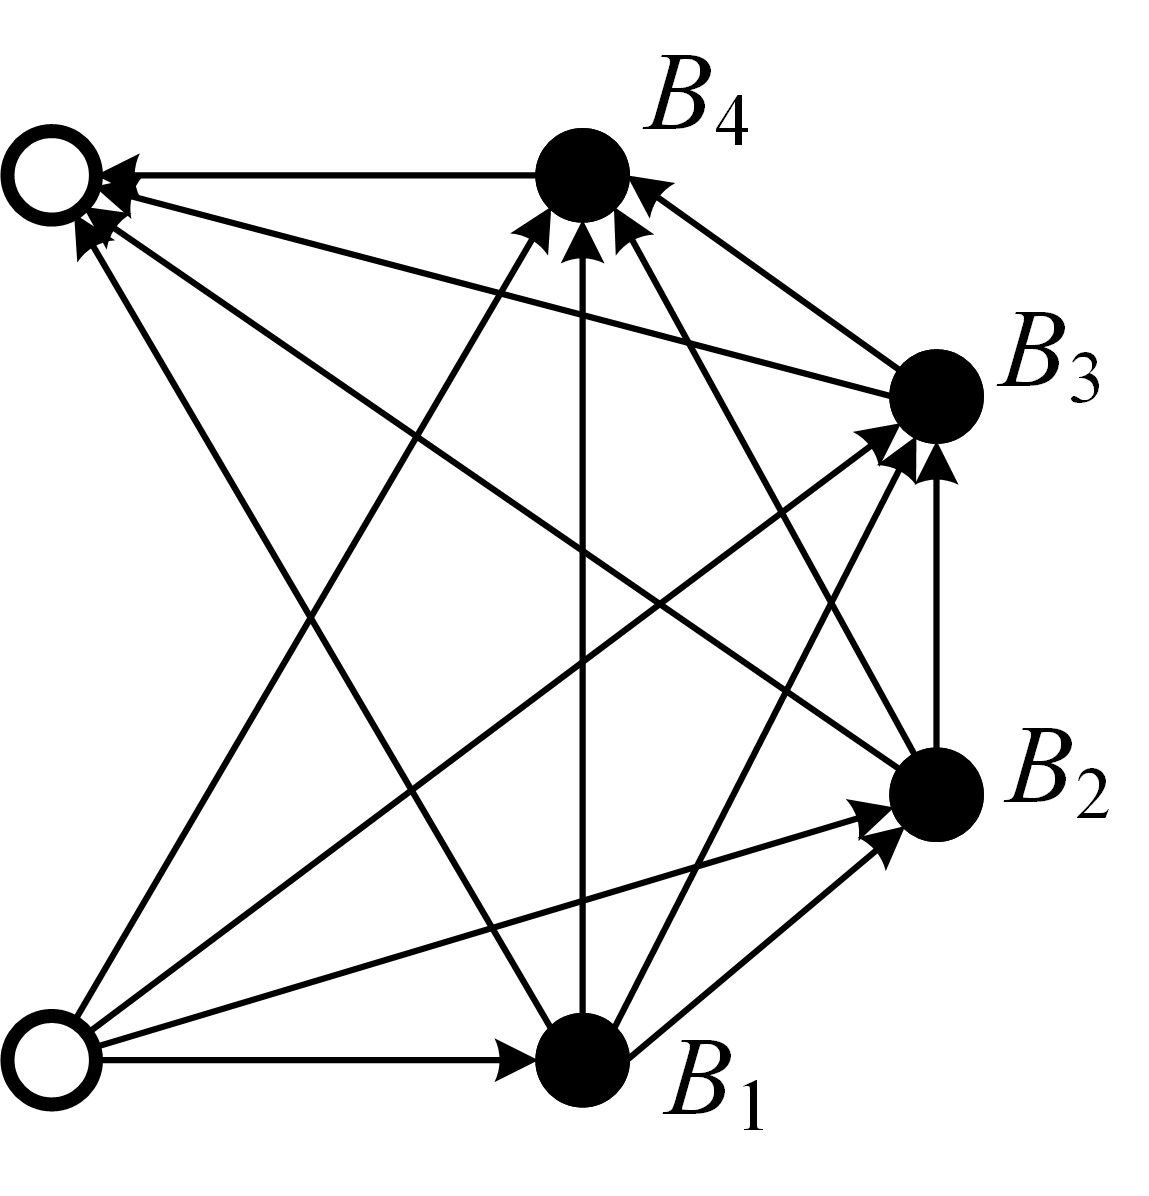
\includegraphics[width=\textwidth]{../attachments/direct-graph-he.png}
        \caption{}
        \label{fig:direct-graph-he}
    \end{subfigure}
    \hspace{0.02\textwidth}
    \begin{subfigure}[b]{0.23\textwidth}
        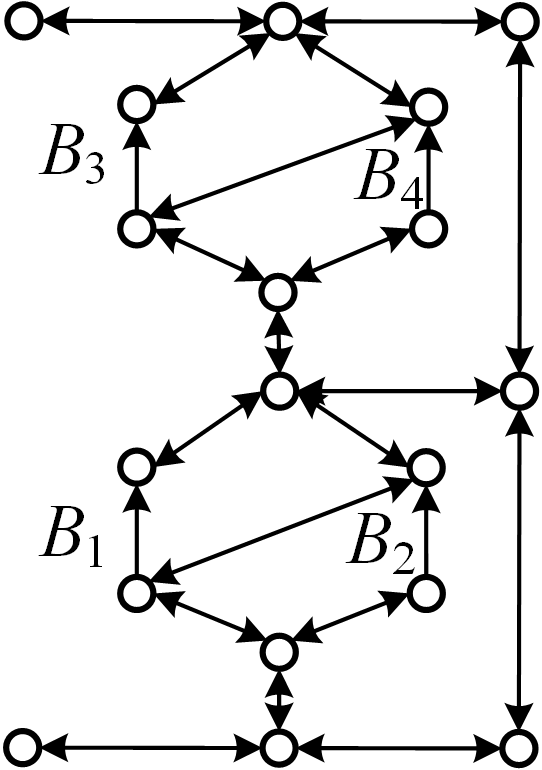
\includegraphics[width=\textwidth]{../attachments/direct-graph-xu.png}
        \caption{}
        \label{fig:direct-graph-xu}
    \end{subfigure}
    \hspace{0.02\textwidth}
    \begin{subfigure}[b]{0.24\textwidth}
        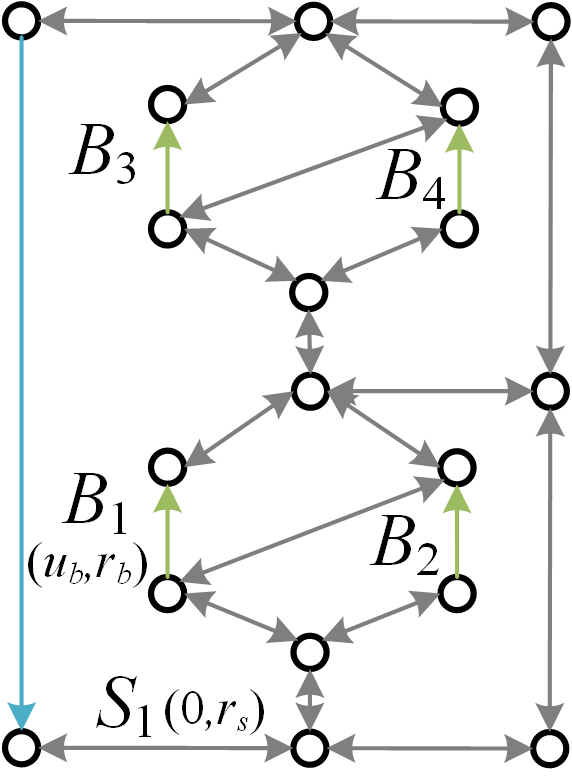
\includegraphics[width=\textwidth]{../attachments/direct-graph-my.png}
        \caption{}
        \label{fig:direct-graph-my}
    \end{subfigure}
    \\
    \begin{subfigure}[b]{0.8\textwidth}
        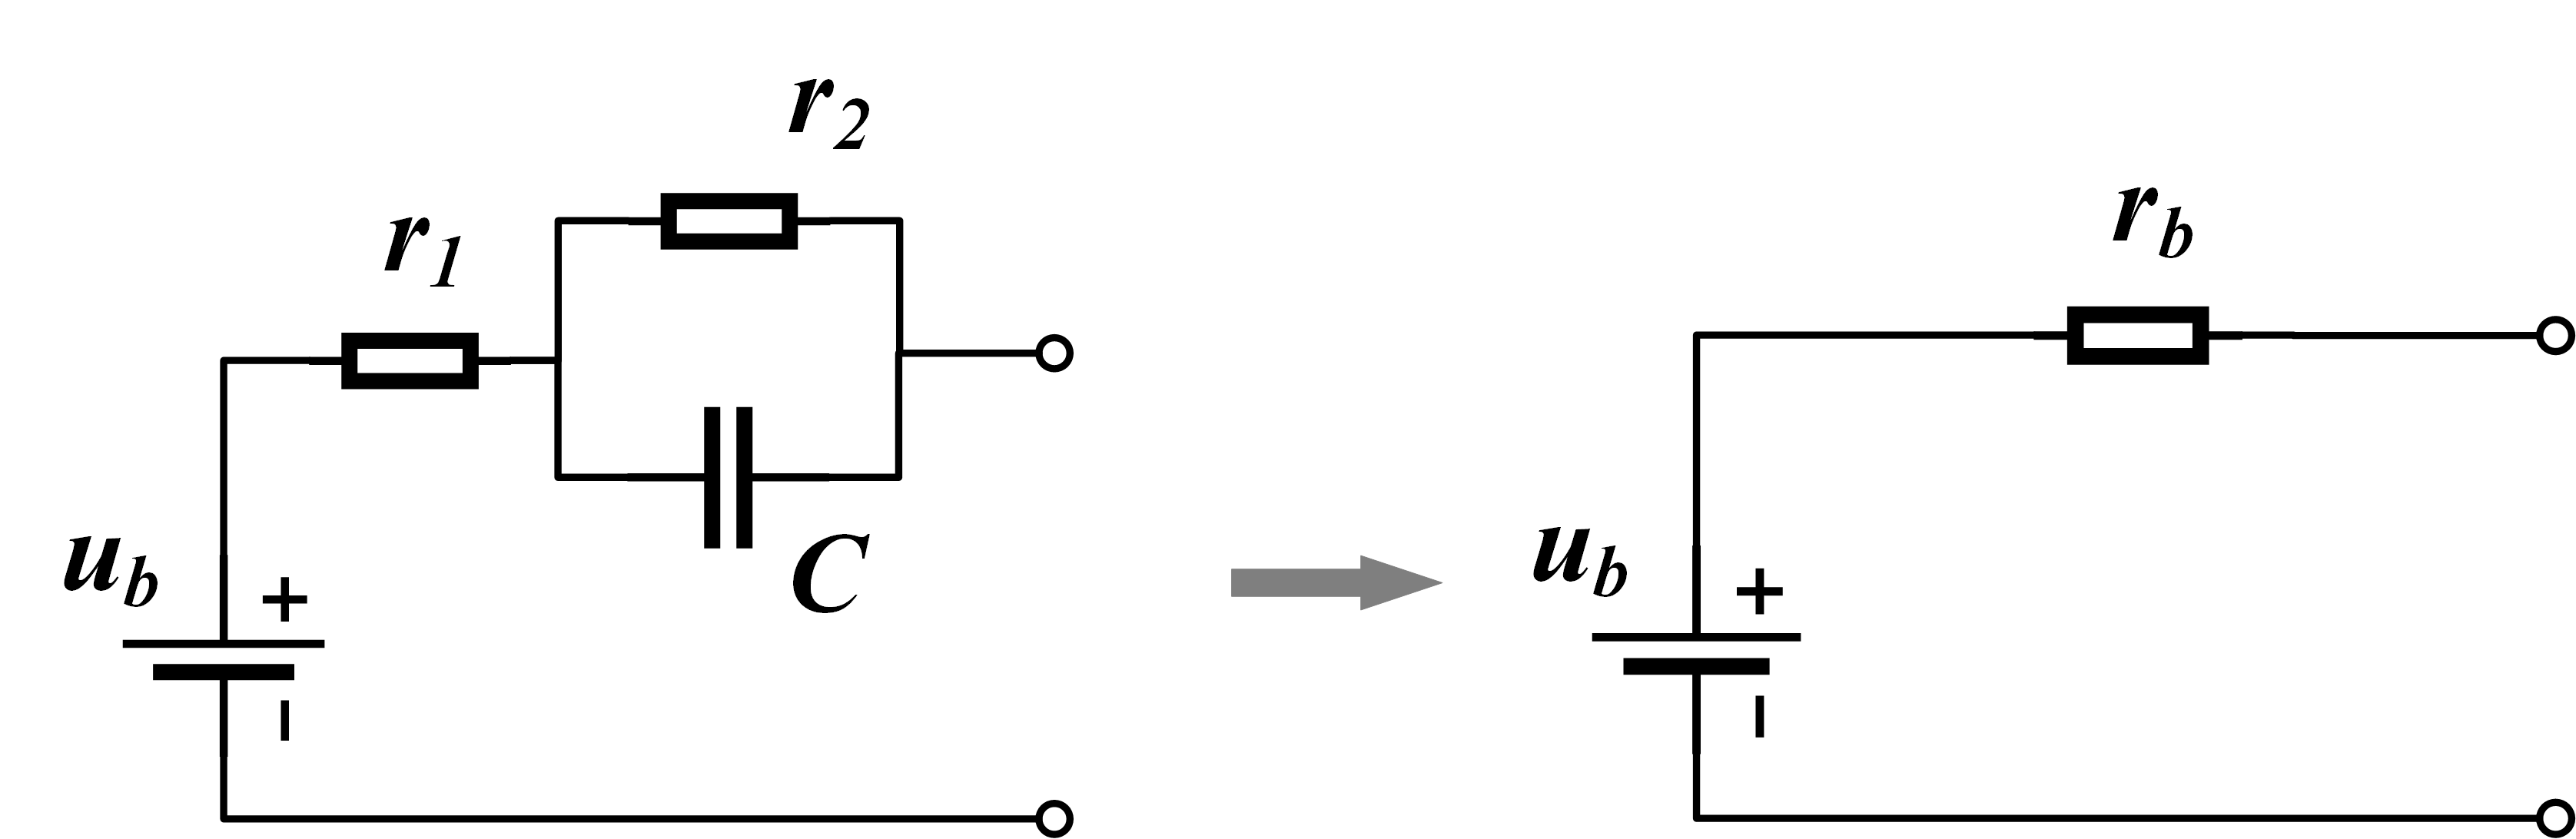
\includegraphics[width=\textwidth]{../attachments/battery_simple.png}
        \caption{}
        \label{fig:battery_simple}
    \end{subfigure}
    \caption{ 
        Directed graph models used in (a) He's work \cite{heExploringAdaptiveReconfiguration2013}, (b) our previous work , and (c) this paper.
        (d) The equivalent circuit of a battery in this method.
    }
\end{figure}

He et al. \cite{heExploringAdaptiveReconfiguration2013} once proposed an abstracted directed graph model for RBS, where the nodes represented the batteries, the edges represented the configuration flexibility, and the weight of each vertex corresponded to the battery voltage ( Fig. \ref{fig:direct-graph-he}). 
The model effectively captured all potential system configurations and offered a direct metric for configuration flexibility, but it did not specify the physical implementation of the connectivity between batteries, meaning one graph might have had multiple RBS structures.
We previously proposed a novel directed graph model that, in contrast to He's model, used nodes to represent the connections between batteries and switches, and directed edges to represent batteries and switches (Fig. \ref{fig:direct-graph-xu}), allowing for a one-to-one correspondence between the RBS structure and the directed graph model. 
This model was able to accurately and comprehensively represent the RBS topological structure but could not be used for quantitative MAC calculations due to the lack of consideration for battery and switch performance parameters. 
To address this, an improved directed graph model is used here based on our original model, adding electromotive force and resistance attributes on the edges based to equivalent circuits (Fig. \ref{fig:direct-graph-my}).
The model also considers the external load as an equivalent resistance and integrate it into the analysis, making it a complete circuit model for later circuit analysis.
The following will provide a detailed explanation of the method for equating the components in RBS and constructing the directed graph model.


In order to use circuit analysis methods to solve the MAC of the RBS, the components in the RBS are equated to ideal circuit elements.
As shown in Fig. \ref{fig:battery_simple}, the battery in the RBS can be represented as a black-box circuit consisting of two resistors (i.e., $r_1$ and $r_2$) and a capacitor (i.e., $C$), known as the Thevenin model\cite{hongwenheStateofChargeEstimationLithiumIon2011,mousavig.VariousBatteryModels2014}.
With an emphasis on the stable output of the RBS, the capacitor in the Thevenin model can be considered as an open circuit without affecting the steady-state current.
Therefore, the battery $i$ in the RBS can be simplified as the series connection between a constant voltage source $u_{i}$ and a resistor $r_{i}$.
Furthermore, the state of switch $j$ in the RBS is represented by a binary variable $x_j$, where 0 is for ON and 1 is for OFF, respectively.
When the switch is closed, it can be regarded as a resistor with a very small resistance value $r_{j}$.
Lastly, the external load is considered as a resistor with a value of $R_o$.


For a given RBS structure, the directed graph model for the RBS is constructed as a directed graph $G(V,E)$ in such a way that:
\begin{enumerate}
    \item Nodes:
        The nodes in the directed graph correspond to the connection points of components in the actual RBS. 
        Assuming there are a total of $N$ nodes in the RBS, for the sake of convenience, the anode of the RBS is denoted as $v_1$ and the cathode as $v_N$.
    \item Edges:
        The edges in the directed graph correspond to the batteries, switches, and external electrical loads in the actual RBS.
        Therefore, there are three types of directed edges. 
        For a battery $B_i$, its directed edge $e_i$ is drawn from the cathode to the anode, as the battery only allows current to flow in one direction when in operation.
        For a switch $S_j$, since it is allowed to work under bi-directional currents, it is represented by a pair of directed edges with two-way directions. 
        Regarding the external electronic load, as it is connected to the anode and cathode of the RBS, a directed edge from $v_N$ to $v_1$ is used to represent it. 
        In conclusion, for a given RBS structure with $N_b$ batteries and $N_s$ switches, the total number of directed edges is $N_b+2N_s+1$, where 1 refers to the external electrical load.
    \item Edges' attributes:
        Each edge is assigned two attributes, voltage difference and resistance, based on the equivalent method mentioned above.
        The values for the battery $B_i$, switch $S_j$, and external loads correspond to $(u_i, r_i)$, $(0, r_j)$, and $(0, R_o)$, respectively.
\end{enumerate}

\subsection{Constraints and Objective Function}

Based on the definition of MAC, determining the MAC of RBS involves maximizing the RBS output current while ensuring that the currents of all batteries do not exceed the batteries' maximum allowable current. 
In this subsection, the constraints and objective function to solve the RBS's MAC will be established through circuit analysis, based on the previously constructed directed graph model.


First, the topology in the directed graph model is represented in matrix form $\bm{A}$, known as the incidence matrix , to facilitate circuit analysis.
The specific definition of the incidence matrix is shown in Eq. \ref{eq:A}.
\begin{align}\label{eq:A}
    a_{kl}=
    \begin{cases}
        1,  & \text{edge $l$ leaves node $k$},\\
        -1, & \text{edge $l$ enters node $k$},\\
        0,  & \text{otherwise}.
    \end{cases}
\end{align}
For a directed graph consisting of $N$ nodes and $N_b+2N_s+1$ directed edges, its incidence matrix $\bm{A}$ is an $N\times(N_b+2N_s+1)$ matrix. 
In this matrix, the rows and columns represent the nodes and edges of the directed graph, respectively.
By distinguishing the components in the RBS corresponding to each column , $\bm{A}$ can be rewritten as:
\begin{equation}\label{eq:A_bso}
    \bm{A} =
    \begin{bmatrix}
        \bm{A}_b & \bm{A}_s & \bm{A}_o
    \end{bmatrix},
\end{equation}
where $\bm{A}_b$, $\bm{A}_s$ and $\bm{A}_o$ are the sub-matrices corresponding to the batteries, switches and external electrical load, respectively.
To alleviate computational complexity, matrix $\bm{A}$ undergoes dimensionality reduction.
Since each directed edge has one node to leave and one to enter, the sum of the values in every column of $\bm{A}$ is zero.
Therefore removing any single one row will not result in a loss of information. 
Without loss of generality, the last row is removed here.
On the other hand, since each switch in the RBS is represented by a pair of directed edges with two-way directions, the two columns corresponding to the switch are mutually opposite.
Thus, for the sub-matrix $\bm{A}_s$, only one column is retained for each pair of columns representing the same switch.
As a result, $\bm{A}$ can be reduced to a $(N-1)\times(N_b+N_s+1)$ matrix, denoted as $\bm{\tilde{A}}$, for further calculation of current and voltage.
Similar to Eq. \ref{eq:A_bso}, $\bm{\tilde{A}}$ can be rewritten as:
\begin{equation}\label{eq:A_bso_tilde}
    \bm{\tilde{A}} =
    \begin{bmatrix}
        \bm{\tilde{A}}_b & \bm{\tilde{A}}_s & \bm{\tilde{A}}_o
    \end{bmatrix}.
\end{equation}


After obtaining the incidence matrix, the currents of all batteries and output in RBS are determined by solving the circuit equations.
According to Kirchhoffs law, we have
\begin{align}\label{eq:Kirchhoffs_law}
    \begin{cases}
        \bm{\tilde{A}} \bm{I} = \bm{0}, \\
        \bm{U}        = \bm{\tilde{A}}^\T \bm{U}_n,
    \end{cases}
\end{align}
where $\bm{I}$ and $\bm{U}$ indicate the current and voltage difference arrays of the $N_b+N_s+1$ edges, respectively;
$\bm{U}_n$ is the voltage array of the $N-1$ nodes.
These directed edges are treated as generalized branches and expressed in matrix form as follows
\begin{equation}\label{eq:generalized_branches}
    \bm{I} = \bm{Y}\bm{X} \bm{U} - \bm{Y}\bm{X} \bm{U}_s +\bm{I}_s,
\end{equation}
where $\bm{U}_s$ and $\bm{I}_s$ denote the source voltage and source current of the generalized branches, respectively.
Because all batteries have been equivalent to voltage sources rather than current sources in the previous subsection, all elements of the array $\bm{I}_s$ are 0, 
while the elements of the array $\bm{U}_s$ are equal to the first attribute of the corresponding edges in the directed graph.
The $\bm{Y}$ in \ref{eq:generalized_branches} is the admittance matrix of the circuit, defined as the inverse of the impedance matrix.
That is the elements of the diagonal matrix $\bm{Y}$ are equal to the reciprocal of the second attribute of the corresponding edges in the directed graph, and the off-diagonal elements are 0.
The $\bm{X}$ is the state matrix, which describes whether the RBS batteries and switches are allowed to pass current.
It is defined as
\begin{equation}\label{eq:X}
    \bm{X} = \diag(
    \underbrace{1, 0 \cdots, 1}_{N_b~\text{of}~0/1},
    \underbrace{1, 0 \cdots, 1}_{N_s~\text{of}~0/1},
    1)
    =\begin{bmatrix}
        \bm{X}_b & & \\
        & \bm{X}_s &\\
        & & 1
    \end{bmatrix}.
\end{equation}
Where the elements $x_i$ of the matrix $\bm{X}_b$ represent whether the battery $i$ has been removed from the circuit, with $x_i=1$ indicating removal and $x_i=0$ indicating that it is still available to supply power. 
When all batteries are health and capable of providing current to the external load, $\bm{X}_b$ is an identity matrix. 
The elements $x_j$ of the matrix $\bm{X}_s$ represent whether the switch $j$ is closed, with $x_j=1$ indicating closure and $x_j=0$ indicating disconnection, which is consistent with the previous subsection.


Theoretically, the output current $I_o$ and the currents of each battery $\bm{I}_b$ in the RBS  can be determined by solving Eqs. \ref{eq:Kirchhoffs_law}, \ref{eq:generalized_branches}, and \ref{eq:X} under any given state $\bm{X}$.
In order to obtain specific constraint conditions and objective functions, it is further assumed that all batteries have the same electromotive force and internal resistance, denoted as $u_b$ and $r_b$, respectively.
This allows for the derivation of explicit expressions for $I_o$ and $\bm{I}_b$.
After derivation and simplification, the output current $I_o$ and the currents of each battery $\bm{I}_b$ are ultimately represented as Eqs. \ref{eq:I_o} and \ref{eq:I_b}, respectively.
\begin{equation}\label{eq:I_o}
    I_o = \frac{1}{R_o r_b} \bm{\tilde{A}}_o^\T \bm{Y}_n^{-1}(\bm{X}) \bm{\tilde{A}}_b \bm{U}_b,
\end{equation}
\begin{equation}\label{eq:I_b}
    \bm{I}_b = \frac{1}{r_b^2}[\bm{\tilde{A}}_b^\T \bm{Y}_n^{-1}(\bm{X}) \bm{\tilde{A}}_b\bm{U}_b -r_b \bm{U}_b],
\end{equation}
where $\bm{U}_b$ is a $N_b\times 1$ array with all elements equaling to $u_b$;
$\bm{Y}_n$ is the equivalent admittance matrix of the circuit, defined as
\begin{equation}\label{eq:Yn}
    \bm{Y}_n (\bm{X}) = \frac{1}{R_o} \bm{\tilde{A}}_o\bm{\tilde{A}}_o^\T + \frac{1}{r_b} \bm{\tilde{A}}_b\bm{X}_b\bm{\tilde{A}}_b^\T + \frac{1}{r_s}\bm{\tilde{A}}_s\bm{X}_s\bm{\tilde{A}}_s^\T.
\end{equation}


To characterize the current output capacity of the RBS structure under different switching states, an indicator $\eta$ is defined by the ratio of $I_o$ and $\max (\bm{I}_b)$ shown in Eq. \ref{eq:eta}:
\begin{equation}\label{eq:eta}
    \eta = \frac{I_o}{\max (\bm{I}_b)}.
\end{equation}
Finally the problem of solving MAC can be formulated as
\begin{align}
    & \max \eta(\bm{X}_s) \label{eq:max_eta}\\
    \text{s.t.} & \max (\bm{I}_b) \leq I_m, \label{eq:Ib_leq_Im}
\end{align}
where $I_m$ is the maximum allowable current of the battery.


However, it is computationally difficult to solve \ref{eq:max_eta} because of the $\bm{Y}_n^{-1}$.
On one hand, due to the introduction of nonlinear terms by $\bm{Y}_n^{-1}$, many effective methods in linear optimization are not suitable for this problem.
On the other hand, the rank of $Y_{n}$ is proportional to the number of batteries and switches, which can be very large for a large RBS system, leading to significant computational burden.
Therefore, intelligent algorithms that rely on evolving by iteration may face efficiency issues when dealing with large RBS system.
% 如果有时间,可以在案例部分做个对比,看看智能算法和本文算法的效率差距有多大。
In order to address this issue, the problem should be considered from the perspective of guiding the RBS to reconstruct as many parallel structures as possible.
Consequently, a greedy algorithm based on the shortest path is proposed. 
The detailed implementation process is presented in the following two subsections.

% Herein provides the solution procedure of …: 1. 2.
% 考虑这部分怎么写,想不出就直接删了吧。
% The integrability of the matrix $\bm{Y}_n$ is explained here.
% Although the above solution procedure requires the matrix $\bm{Y}_n$ to be invertible, it is still possible to encounter integrable $\bm{Y}_n$ in the calculation.
% The physical meaning of this case corresponds to the fact that due to the excessive number of switches in OFF, the solved circuit structure forms circuit branches independent of the main circuit, i.e., the circuit connected to the anode and cathode of the RBS. 
% Since these independent branches are not connected to the main circuit, the voltage potentials of these branches cannot be determined and theoretically an infinite number of sets of solutions exist. 
% Benfit from the independence, these solutions have no influence on the results of the main circuit. 
% Since only the currents and voltages of the main circuit are of interest, only one of these solutions needs to be chosen for subsequent calculation.

\subsection{Shortest Path}

The path $p$ used in this method is defined as the complete route that passes through one battery (or a consecutive series of batteries) and closed switches, connecting the anode $v_1$ to the cathode $v_N$ of the RBS.
By applying a penalty to the series-connected batteries on the path, where additional batteries imply a longer distance, the algorithm encourages the RBS to form parallel structures as much as possible.
Meanwhile, to reduce the number of switches controlled during the reconstruction process, a penalty is also applied to the total number of switches on the path, while ensuring the minimum number of batteries.
Therefore, the distance $\omega$ of the path $p$ is defined by the following equation: 
\begin{equation}\label{eq:weight}
    \omega(p) = N_s \cdot n_b (p) + n_s (p),
\end{equation}
where $N_s$ is the total number of switches in the system; 
$n_b(p)$ and $n_s(p)$ are number of batteries and switches in the path $p$ respectively. 
Moreover, the shortest path $SP_i$ is defined as the path with the minimum $\omega$ for battery $i$, as shown in the following equation:
\begin{equation}\label{eq:def_sp}
    SP_i = \mathop{\arg\min}_{p \in P_i} \omega(p),
\end{equation}
where $P_i$ is the set of all paths from $v_1$ to $v_N$ which pass through the directed edge $i$.


The $SP_i$ can be solved by the Dijkstra algorithm.
The Dijkstra algorithm is a graph search method that finds the shortest path between two given nodes in a weighted graph, efficiently solving the single-source shortest path problem.
Assuming that the cathode and anode of battery $i$ are denoted as $v_i^-$ and $v_i^+$ respectively, the path $p$ of battery $i$  can be divided into three segments : $v_1 \rightarrow v_i^-$, $v_i^+ \rightarrow v_N$, and $v_i^- \rightarrow v_i^+$.
The $v_i^- \rightarrow v_i^+$ is the directed edge corresponding to battery $i$. 
With the Dijkstra algorithm, shortest paths for the $v_1 \rightarrow v_i^-$ and $v_i^+ \rightarrow v_N$ can be calculated under the weights given in Eq. \ref{eq:weight}, denoted as $SP(v_i^- \rightarrow v_i^+)$ and $SP(v_i^+ \rightarrow v_N)$, respectively.
Finally, the $SP_i$ for battery $i$ is formed by the complete path with $SP(v_1 \rightarrow v_i^-)$, $v_i^- \rightarrow v_i^+$, and $SP(v_i^+ \rightarrow v_N)$.

\subsection{Greedy Algorithm}\label{subsec:greedy_solution}

From the perspective of series/parallel, the more batteries are connected into circuit via their $SP$s, the more batteries are connected in parallel.

In this subsection, a greedy algorithm is proposed based on shortest paths ($SP$s), which is given here firstly. % 这句话改成 greedy algorithm 在整个 MAC 计算中的作用

% 说明 利用 SP 求解 MAC 的原理
Since batteries can provide more total output current when connected in parallel than in series, the algorithm greedily selects as many cells as possible to be connected into to the overall circuit via their $SP$s to obtain the MAC.
% the maximu....SP.....I(两句话合到一起); 这种并联结构可以通过贪心算法得到;

% 贪心算法的具体步骤
The dichotomy method is also performed to faster find the right number of $SP$s. % 添加对贪心算法的步骤介绍,具体某一步说明采用了二分法…
% 二分法融入贪心算法,添加贪心算法步骤
After finding the potential SPs combinations in correspondence MAC, the state variable $\bm{X}_s$ of the switches can be determined, and the optimization problem \ref{eq:max_eta} can be solved using Eq. \ref{eq:eta}, \ref{eq:I_o} and \ref{eq:I_b}.
The overall flowchart is shown in Fig. \ref{fig:flowchart}, and the corresponding pseudo-code of the algorithm is shown in Appendix \ref{alg:eta_RBS}. % 这句话应该放前面说,采用“总-分”架构,先给出流程图,然后再结合流程各步骤介绍每类具体算法的应用过程

\tikzset{
  meta box/.style={draw, black, very thick, text centered, },
  punkt/.style={meta box, rectangle, rounded corners, inner sep=.25em, minimum height=2em, minimum width=4em, align=center, text width=10em },
  round/.style={meta box, circle, minimum size=0, inner sep=0pt, outer sep=0pt },
  every fit/.style={draw, thick, dashed, gray, inner xsep=.5em, inner ysep=.75em }
}
\begin{figure}
\begin{tikzpicture}[font=\small, node font=\small, node distance=1.5em]
    \node[punkt]     (input) {Input: RBS structure};
    \node[punkt, below=0.3of input] (get_SP) {get $SP$s by Eqs. \ref{eq:weight} and \ref{eq:def_sp} and Dijkstra Search};
    \node[punkt, below=0.3of get_SP] (get_A) {get $\bm{A}$ from Eq. \ref{eq:A}};
    \node[punkt, below=0.3of get_A] (get_Nset) {init $N_{set}=N_b$ };
    \node[punkt, below=0.3of get_Nset] (get_cb) {get $c_b$s by combinating $N_{set}$ batteries from $N_b$};
    \node[draw, diamond, aspect=2, below=0.3of get_cb] (is_check_all_cb) {are all $c_b$s checked?};
    \node[draw, diamond, aspect=2, right=1of is_check_all_cb] (is_Nset_converged) {is $N_{set}$ converged?};
    \node[punkt, above=of is_Nset_converged] (reset_Nset) {reset $N_{set}$ by dichotomy};
    \node[punkt, text width=15em, below=0.3of is_check_all_cb] (get_Xs) {
        select an unchecked $c_b$, and get its $\bm{X}_m$ by \\ 
        if switch $j$ $\in \bigcup_{i\in c_b}SP_i$:\\
        $\bm{X}[j]=1$ else $0$};
    \node[punkt, below=0.3of get_Xs] (get_Yn) {get $\bm{Y}_n$ by Eq.\ref{eq:Yn}};
    \node[draw, diamond, aspect=2, below=0.3of get_Yn] (is_Yn_invertible) {is $\bm{Y}_n$ invertible?};
    \node[punkt, right=1.3of is_Yn_invertible] (construct) {construct an effective solution};
    \node[punkt, below=0.3of is_Yn_invertible] (get_I) {get $I_o$ and $\bm{I}_b$ by Eqs. \ref{eq:I_o} and \ref{eq:I_b}};
    \node[draw, diamond, aspect=2, below=0.3of get_I] (is_leq_Im) {is $\max \bm{I}_b \leq I_m$?};
    \node[punkt, right=1.3of is_leq_Im] (drop_eta) {drop this $\eta$};
    \node[punkt, below=0.3of is_leq_Im] (get_eta) {get $\eta$ by Eq.\ref{eq:eta}};
    \node[punkt, below=0.3of get_eta] (update_max_eta) {update $\max \eta$};
    \node[punkt, right=1of is_Nset_converged] (output) {Output: $\max \eta$};
    \node[round,left=1.5of update_max_eta](point1){};

    \graph{
      (input) -> (get_SP) -> (get_A) -> (get_Nset) -> (get_cb) -> (is_check_all_cb) ->["No"] (get_Xs) -> (get_Yn) -> (is_Yn_invertible) ->["Yes"] (get_I) -> (is_leq_Im) ->["Yes"] (get_eta) -> (update_max_eta);
      (is_check_all_cb) ->["Yes"] (is_Nset_converged) ->["No"] (reset_Nset) -> (get_cb);
      (is_Yn_invertible) ->["No"] (construct) ->[to path={|- (\tikztotarget)}] (get_I);
      (is_leq_Im) ->["No"] (drop_eta) ->[to path={|- (\tikztotarget)}] (update_max_eta);
      (is_Nset_converged) ->["Yes"] (output);
      (update_max_eta) -- (point1) ->[to path={|- (\tikztotarget)}] (is_check_all_cb);
    };
\end{tikzpicture}
\caption{The computational flowchart of the MAC if an RBS.}\label{fig:flowchart}
\end{figure}

\section{Case Study}

% 案例分析部分要点
% - 考虑给个新结构,让MAC=4
% - 直接给出结构的结果(一个我们提出的,模型的边和结点、SP结果示意图、结果表格;其余结构的结果表格)(注意一些表格的caption)
%   - It is composed of a total of 19 nodes and 43 edges. 再分别给出哪些节点、边代表什么
% - eta 反映了结构本身输出电流的能力,与 Io相比
% - MAC 越高越好 (MAC 是一个结构的输出电流上限,越大意味着可输出的范围越大)
% - 电池隔离后 MAC 的变化,评判结构的优劣(多放一些结构)




In this section, an intricate structure shown in Fig. 4 is constructed based on the combination of two RBS structures, which are plotted in Fig. (a) and (b) respectively. 
… % 介绍组成RBS结构的优缺点
The new proposed RBS structure integrates the advantages of these two traditional RBS structures, and is particularly used to demonstrate the use of the proposed MAC determination method.


\subsection{Determination of a new RBS structure}

\begin{figure}[htbp]
    \centering
    \begin{subfigure}[b]{0.45\textwidth}
        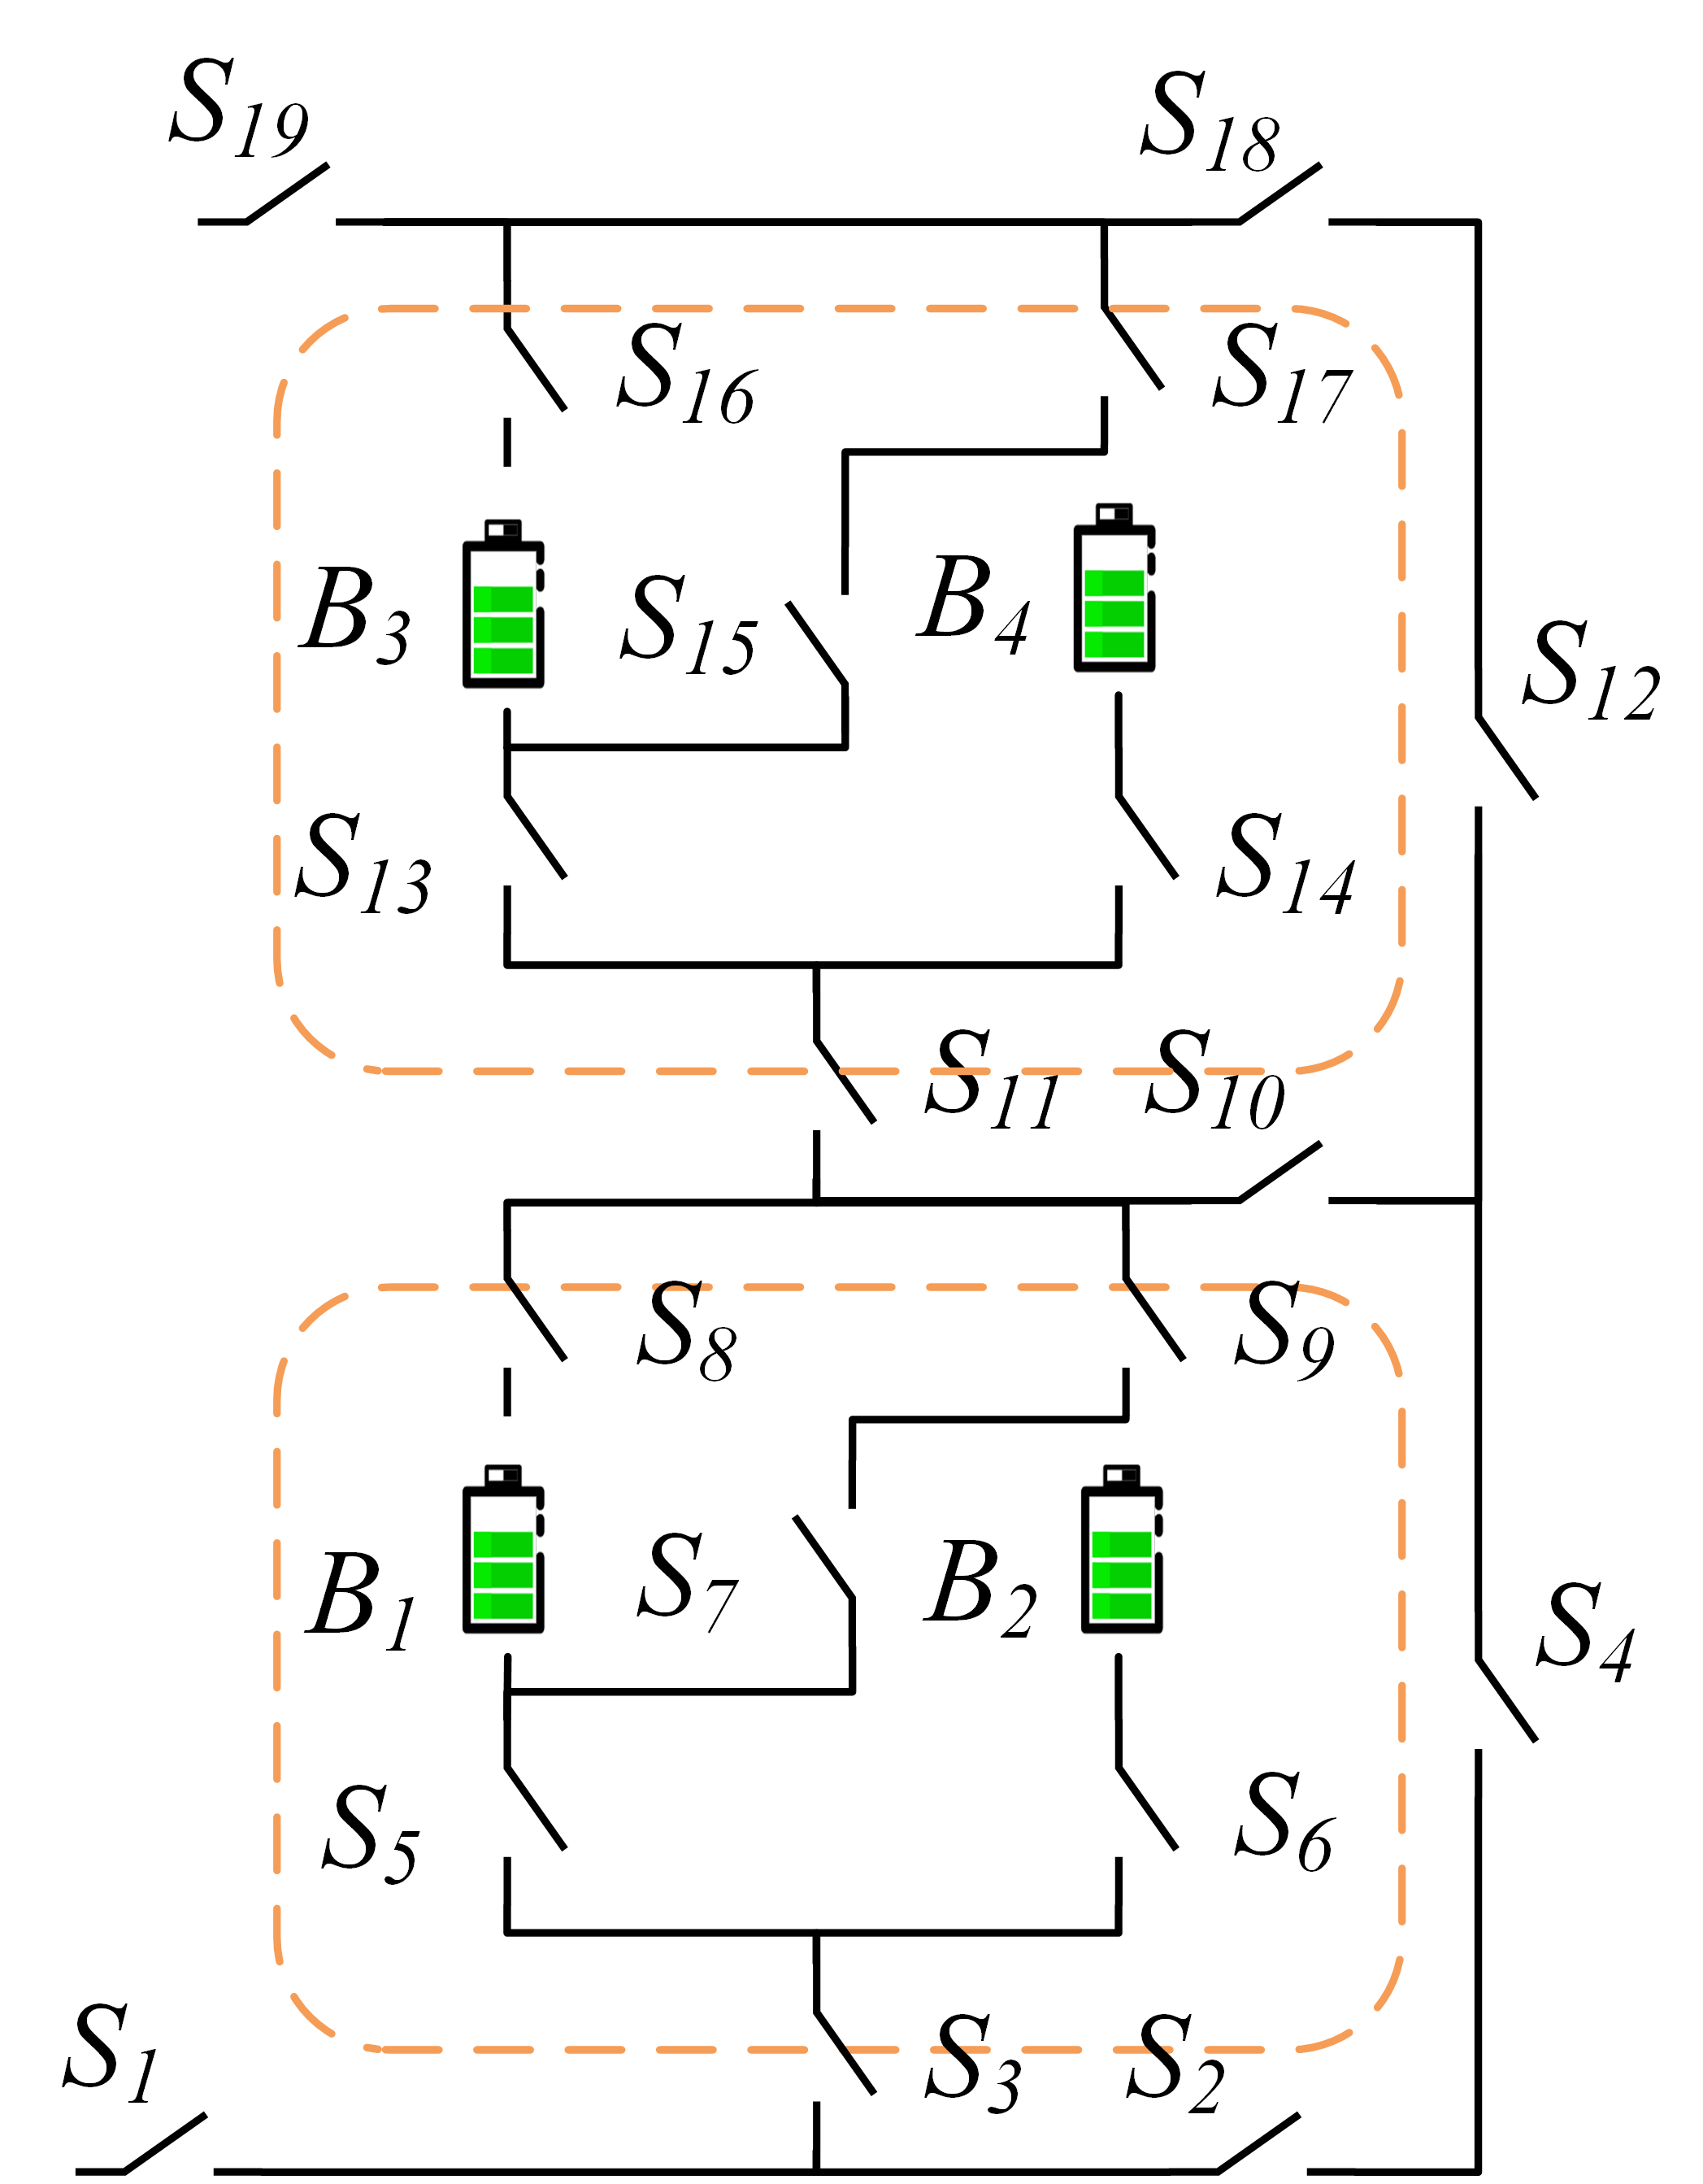
\includegraphics[width=\textwidth]{../attachments/arch-ef.png}
        \caption{}
        \label{fig:arch-ef}
    \end{subfigure}
    \hspace{0.05\textwidth}
    \begin{subfigure}[b]{0.45\textwidth}
        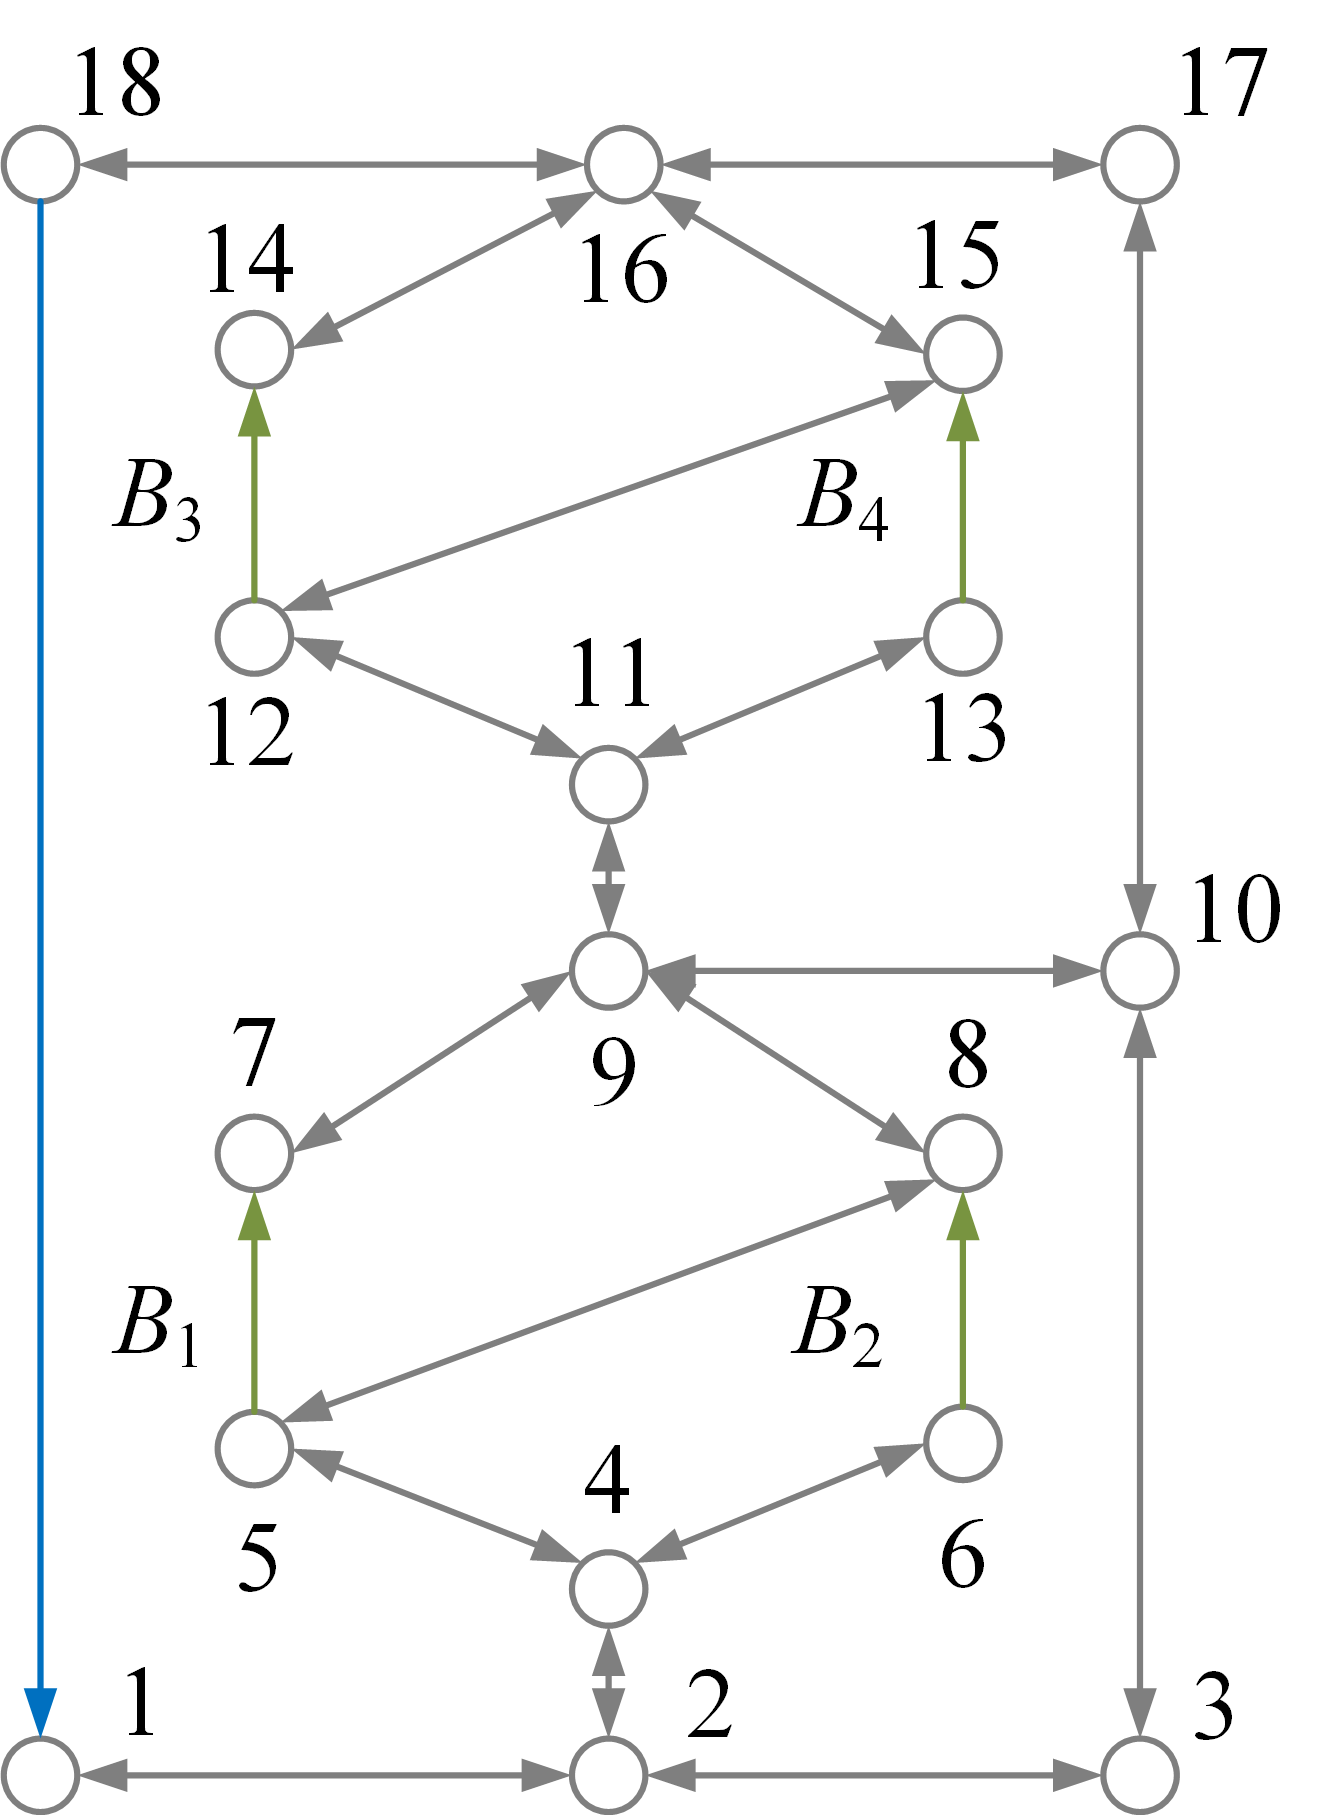
\includegraphics[width=\textwidth]{../attachments/ef-topo.png}
        \caption{}
        \label{fig:ef-topo}
    \end{subfigure}
    \caption{
        (a) The new RBS structure proposed  by ... % 参考正文修改这里
        (b) The corresponding topologic model of the new RBS structure, which is a directed graph.
        % 以下句子放正文
        The nodes represent the connection points of the battery cells and/or the switches.
        The green,gray and blue directed edges represent the battery cells, the switches and the external electrical load, respectively.
    }
\end{figure}

% 以下这段话融入到前一句,分别介绍新建 RBS 结构的两个组成怎么来的, 有什么优点
The RBS structure proposed by Lawson et al\cite{lawsonSoftwareConfigurableBattery2012}, shown in Fig. \ref{fig:arch-e}, easily enables the isolation of the highly degraded battery ( or a series connection of batteries) from the battery module.
In contrast, the structure proposed by Visairo et al\cite{visairoReconfigurableBatteryPack2008}, shown in Fig. \ref{fig:arch-f}, allows the flexibility to switch the cells between series, parallel and mixed series-parallel modes, thus allowing dynamic voltage adjustment according to the external load and improving energy conversion efficiency, but is not as simple as the structure by Lawson et al in terms of isolating cells or adding redundancy. % 这句话太长了
In order to combine the advantages of both above RBS structures, a new structure is obtained by integrating the Visairo RBS structure into Lawson RBS structure as shown in Fig. \ref{fig:arch-ef}.
In this way, the circuit topology of the substructure (for instance the batteries B1, B2 and their related switches) can be changed to enable dynamic and flexible voltage tuning in terms of the external load, as well as taking advantage of the ease of battery isolation and increased redundancy of the main frame.

\subsection{Result}
% 删去太细节的计算

The directed graph in Fig. \ref{fig:ef-topo} represents the topology of the new RBS structure proposed in this study (Fig. \ref{fig:arch-ef}). 
% 下面这句 It is composed of a total of 19 nodes and 43 edges. 先总体介绍模型包括多少个节点和边,再分别给出哪些节点/边代表哪些东西 
In this model, batteries $B_1$, $B_2$, $B_3$, and $B_4$ are represented by green directed edges in the graph, while 19 switches are represented by gray directed edges with two-way directions. 
The external electrical load is considered as a directed edge from the cathode of the RBS (i.e. node 18 ) to the anode (i.e. node 1 ), represented as the blue directed edge in the graph.


Based on the node-edge relationship given in Fig. \ref{fig:ef-topo}, the incidence matrix $\bm{A}$ can be obtained according to Eq. \ref{eq:A}:
\begin{equation}
    \bm{A} = 
    \begin{bmatrix}
        \bm{A}_b & \bm{A}_s & \bm{A}_o
    \end{bmatrix},
\end{equation}

\begin{equation}
    \bm{A}_b^\T = 
    \begin{bmatrix}
        0 & 0 & 0 & 0 & 1 & 0 &-1 & 0 & 0 & 0 & 0 & 0 & 0 & 0 & 0 & 0 & 0 \\
        0 & 0 & 0 & 0 & 0 & 1 & 0 &-1 & 0 & 0 & 0 & 0 & 0 & 0 & 0 & 0 & 0 \\
        0 & 0 & 0 & 0 & 0 & 0 & 0 & 0 & 0 & 0 & 0 & 1 & 0 &-1 & 0 & 0 & 0 \\
        0 & 0 & 0 & 0 & 0 & 0 & 0 & 0 & 0 & 0 & 0 & 0 & 1 & 0 &-1 & 0 & 0 \\
    \end{bmatrix},
\end{equation}

\begin{equation}
    \bm{A}_s^\T = 
    \begin{bmatrix}
        1 &-1 & 0 & 0 & 0 & 0 & 0 & 0 & 0 & 0 & 0 & 0 & 0 & 0 & 0 & 0 & 0 \\
        0 & 1 &-1 & 0 & 0 & 0 & 0 & 0 & 0 & 0 & 0 & 0 & 0 & 0 & 0 & 0 & 0 \\
        0 & 1 & 0 &-1 & 0 & 0 & 0 & 0 & 0 & 0 & 0 & 0 & 0 & 0 & 0 & 0 & 0 \\
        0 & 0 & 1 & 0 & 0 & 0 & 0 & 0 & 0 &-1 & 0 & 0 & 0 & 0 & 0 & 0 & 0 \\
        0 & 0 & 0 & 1 &-1 & 0 & 0 & 0 & 0 & 0 & 0 & 0 & 0 & 0 & 0 & 0 & 0 \\
        0 & 0 & 0 & 1 & 0 &-1 & 0 & 0 & 0 & 0 & 0 & 0 & 0 & 0 & 0 & 0 & 0 \\
        0 & 0 & 0 & 0 & 1 & 0 & 0 &-1 & 0 & 0 & 0 & 0 & 0 & 0 & 0 & 0 & 0 \\
        0 & 0 & 0 & 0 & 0 & 0 & 1 & 0 &-1 & 0 & 0 & 0 & 0 & 0 & 0 & 0 & 0 \\
        0 & 0 & 0 & 0 & 0 & 0 & 0 & 1 &-1 & 0 & 0 & 0 & 0 & 0 & 0 & 0 & 0 \\
        0 & 0 & 0 & 0 & 0 & 0 & 0 & 0 & 1 &-1 & 0 & 0 & 0 & 0 & 0 & 0 & 0 \\
        0 & 0 & 0 & 0 & 0 & 0 & 0 & 0 & 1 & 0 &-1 & 0 & 0 & 0 & 0 & 0 & 0 \\
        0 & 0 & 0 & 0 & 0 & 0 & 0 & 0 & 0 & 1 & 0 & 0 & 0 & 0 & 0 & 0 &-1 \\
        0 & 0 & 0 & 0 & 0 & 0 & 0 & 0 & 0 & 0 & 1 &-1 & 0 & 0 & 0 & 0 & 0 \\
        0 & 0 & 0 & 0 & 0 & 0 & 0 & 0 & 0 & 0 & 1 & 0 &-1 & 0 & 0 & 0 & 0 \\
        0 & 0 & 0 & 0 & 0 & 0 & 0 & 0 & 0 & 0 & 0 & 1 & 0 & 0 &-1 & 0 & 0 \\
        0 & 0 & 0 & 0 & 0 & 0 & 0 & 0 & 0 & 0 & 0 & 0 & 0 & 1 & 0 &-1 & 0 \\
        0 & 0 & 0 & 0 & 0 & 0 & 0 & 0 & 0 & 0 & 0 & 0 & 0 & 0 & 1 &-1 & 0 \\
        0 & 0 & 0 & 0 & 0 & 0 & 0 & 0 & 0 & 0 & 0 & 0 & 0 & 0 & 0 & 1 &-1 \\
        0 & 0 & 0 & 0 & 0 & 0 & 0 & 0 & 0 & 0 & 0 & 0 & 0 & 0 & 0 & 1 & 0 \\
    \end{bmatrix},
\end{equation}

\begin{equation}
    \bm{A}_o^\T = 
    \begin{bmatrix}
       -1 & 0 & 0 & 0 & 0 & 0 & 0 & 0 & 0 & 0 & 0 & 0 & 0 & 0 & 0 & 0 & 0 \\
    \end{bmatrix}.
\end{equation}
The state matrix $\bm{X}$ is determined by the switches' state, that is, the specific configuration of the RBS.
For example, when switch $S_1$, $S_3$, $S_5$, $S_6$, $S_8$, $S_9$, $S_{11}$, $S_{13}$, $S_{14}$, $S_{16}$, $S_{17}$ and $S_{19}$ are ON, and the rest of the switches are OFF, the state matrix $\bm{X}$ is given by
\begin{equation}
    \bm{X} = diag(
    \underbrace{1,0,1,0,1,1,0,1,1,0,1,0,1,1,0,1,1,0,1}_{\text{switches}},
    \underbrace{1,1,1,1}_{\text{batteries}},
    1
    ).
\end{equation}
By substituting the above specific values of $\bm{A}$ and $\bm{X}$ above into Eqs. \ref{eq:Yn}, \ref{eq:I_o}, \ref{eq:I_b} and \ref{eq:eta} in turn, the $\eta$ at the current situation, i.e. battery cell $B_1$ and $B_2$, $B_3$ and $B_4$ are connected in parallel with each other, and then connected in series to supply the external electrical appliance, can be obtained after the sequential calculation.
The results are shown in Tab. \ref{tab:given_x}.

\begin{table}[htbp]
  \centering
    \caption{Calculating result of the output current $I_o$, battery current $\bm{I}_b$ and ratio $\eta$ for a specificed switches state $\bm{X}_m$ in the structure combining Lawson et al.\cite{lawsonSoftwareConfigurableBattery2012} and Visairo et al.\cite{visairoReconfigurableBatteryPack2008} with 4 battery cells and 19 switches.} % 修改该caption
    \begin{tabular}{cc}
    \toprule
        Structure & 4 battery cells and 19 switches  \\
        % Structure & combining Lawson et al.\cite{lawsonSoftwareConfigurableBattery2012} and Visairo et al.\cite{visairoReconfigurableBatteryPack2008} with 4 battery cells and 19 switches  \\
    \midrule
    Switch ON & 1,3,5,6,8,9,11,13,14,16,17,19 \\
        $\bm{X}_s$ & $\diag(1,0,1,0,1,1,0,1,1,0,1,0,1,1,0,1,1,0,1)$ \\
    \midrule
        $I_o$ & $2u_b/(R_o+r_b)$ \\
        $\bm{I}_b$ & $[u_b/(R_o+r_b),u_b/(R_o+r_b),u_b/(R_o+r_b),u_b/(R_o+r_b)]$ \\
        $\eta$     & 2 \\
    \bottomrule
    \end{tabular}%
  \label{tab:given_x}%
\end{table}%

The above gives the procedure for calculating the current and $\eta$ when the specified switches are given ON or OFF.
However, in order to calculate the MAC of the structure, i.e. the maximum $\eta$, it is necessary to find the corresponding switch state using a greedy strategy, as mentioned in subsection \ref{subsec:greedy_solution}. % 重写这句话,有误解


% 删减以下这段话,不需要单纯描述过程,直接给出结果
Firstly, the weight $N_s$ in Eq. \ref{eq:weight} represents the total number of switches in the system, which is 19. 
By using this formula and the Dijkstra search strategy, the $SP$s of each cell can be obtained, as shown in Figs. \ref{fig:sp1} to \ref{fig:sp4}.
According to the greedy strategy, as many $SP$s as possible should be selected to get the MAC. 
In the first iteration, the $SP$s of all four batteries are selected, and the switch states on the paths are set to ON. 
The corresponding $\bm{X}_s$ are calculated using the previous method, and the currents of the batteries are obtained as $u_b/r_b$, $u_b/r_b$, $u_b/r_b$, and $u_b/r_b$. 
Since all batteries are short-circuited and the current of the battery exceeds the maximum allowed current $I_m$, this solution does not satisfy constraint \ref{eq:Ib_leq_Im} and is discarded. 
The second iteration is carried out using the dichotomy method, and two batteries are selected for the combination. 
Assuming that the selected combinations are $(B1, B2)$, the $\bm{X}_s$ obtained according to the $SP$s are substituted into the previous calculation, and the current of each battery is $u_b/r_b$, $u_b/r_b$, $0$, and $0$. 
This solution meets the condition. 
After that, the case of selecting three cells is considered. 
By similar calculations, it is determined that all solutions do not satisfy the constraint when three cells are selected. 
Finally, the MAC of this structure is $\eta=2$, and the related result is shown in Fig. \ref{fig:ef-mac} and Tab. \ref{tab:find_mac}.

\begin{figure}[htbp]
    \centering
    \begin{subfigure}[b]{0.45\textwidth}
        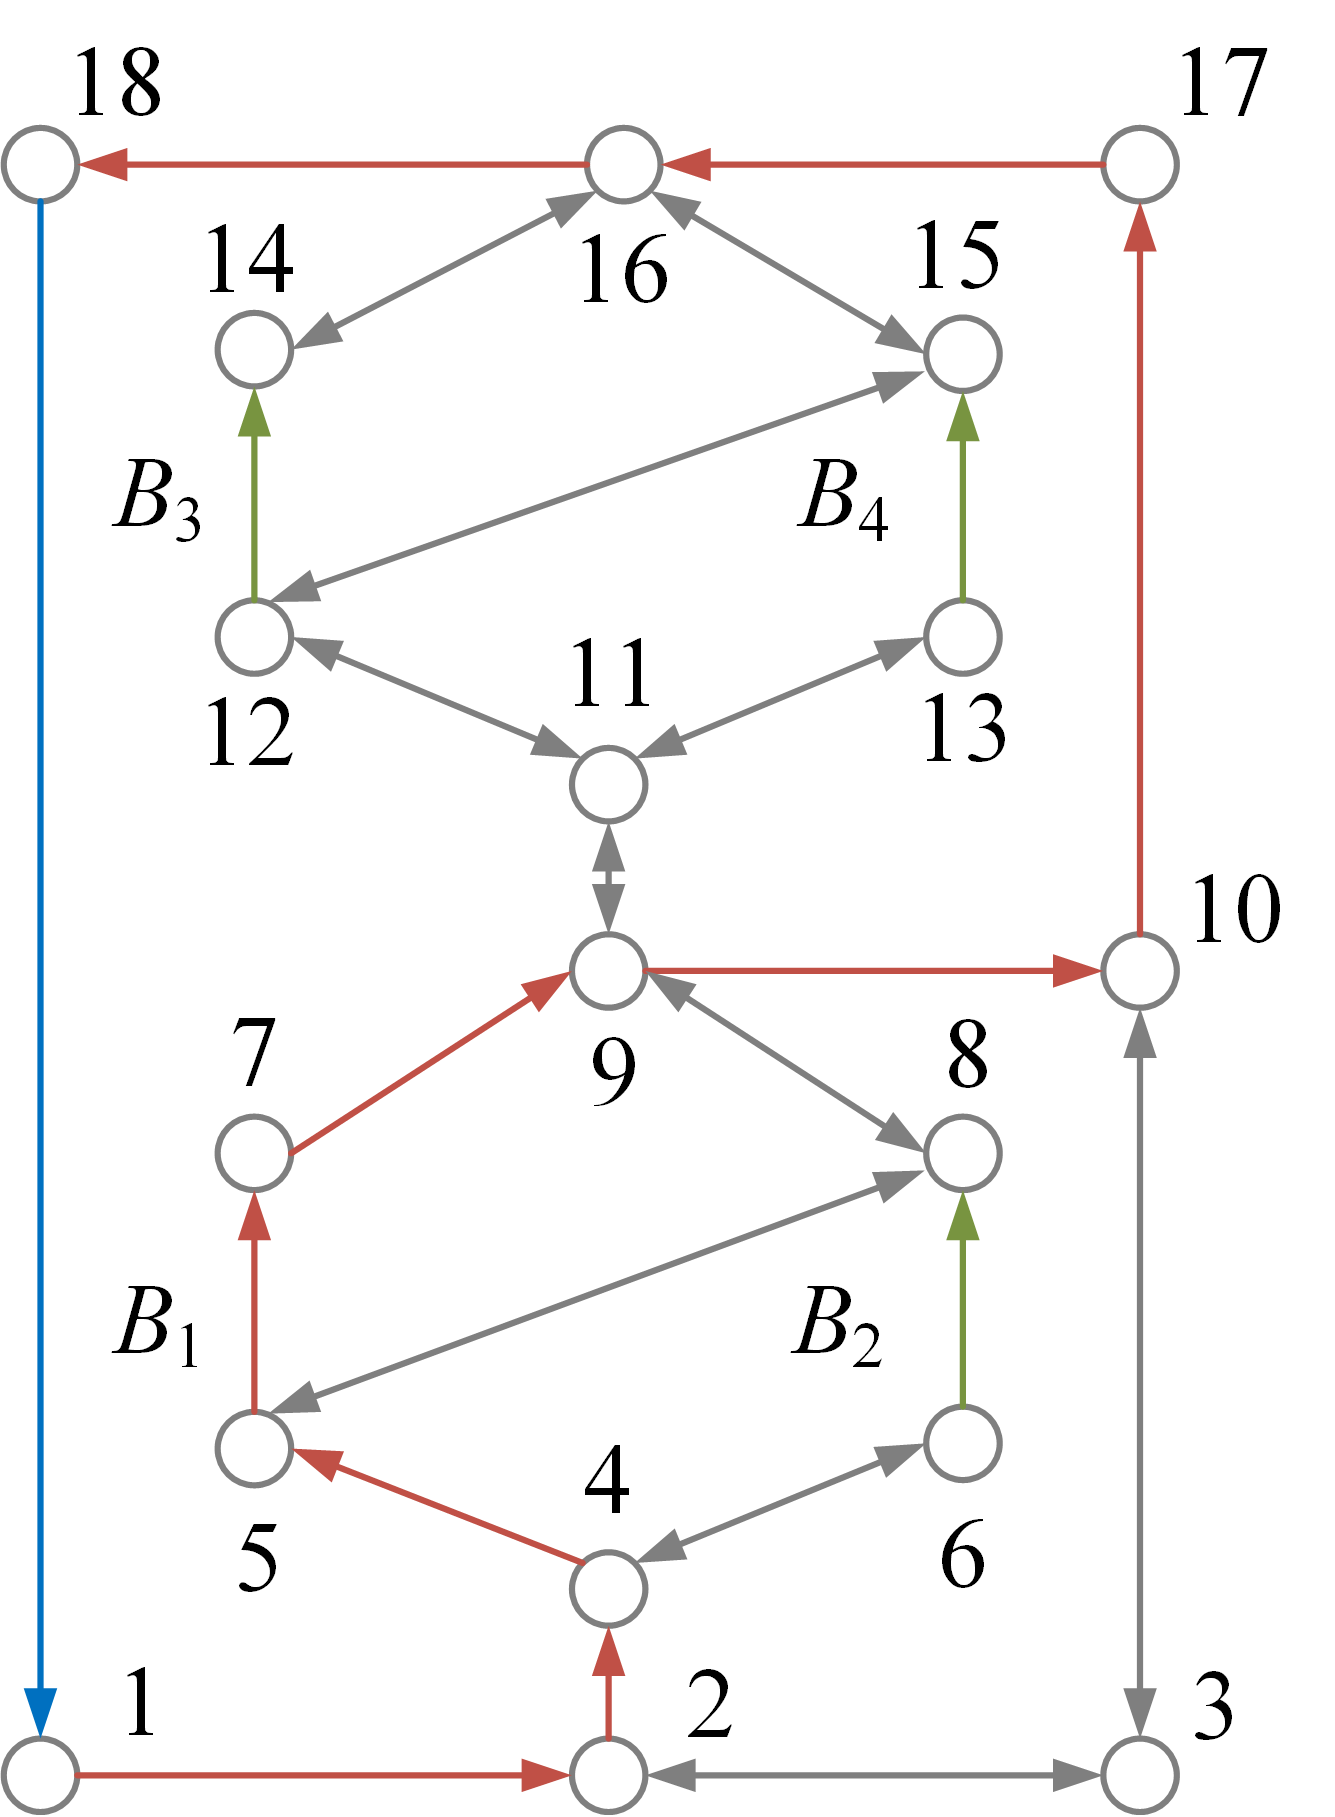
\includegraphics[width=\textwidth]{../attachments/ef-sp1.png}
        \caption{}
        \label{fig:sp1}
    \end{subfigure}
    \hspace{0.05\textwidth}
    \begin{subfigure}[b]{0.45\textwidth}
        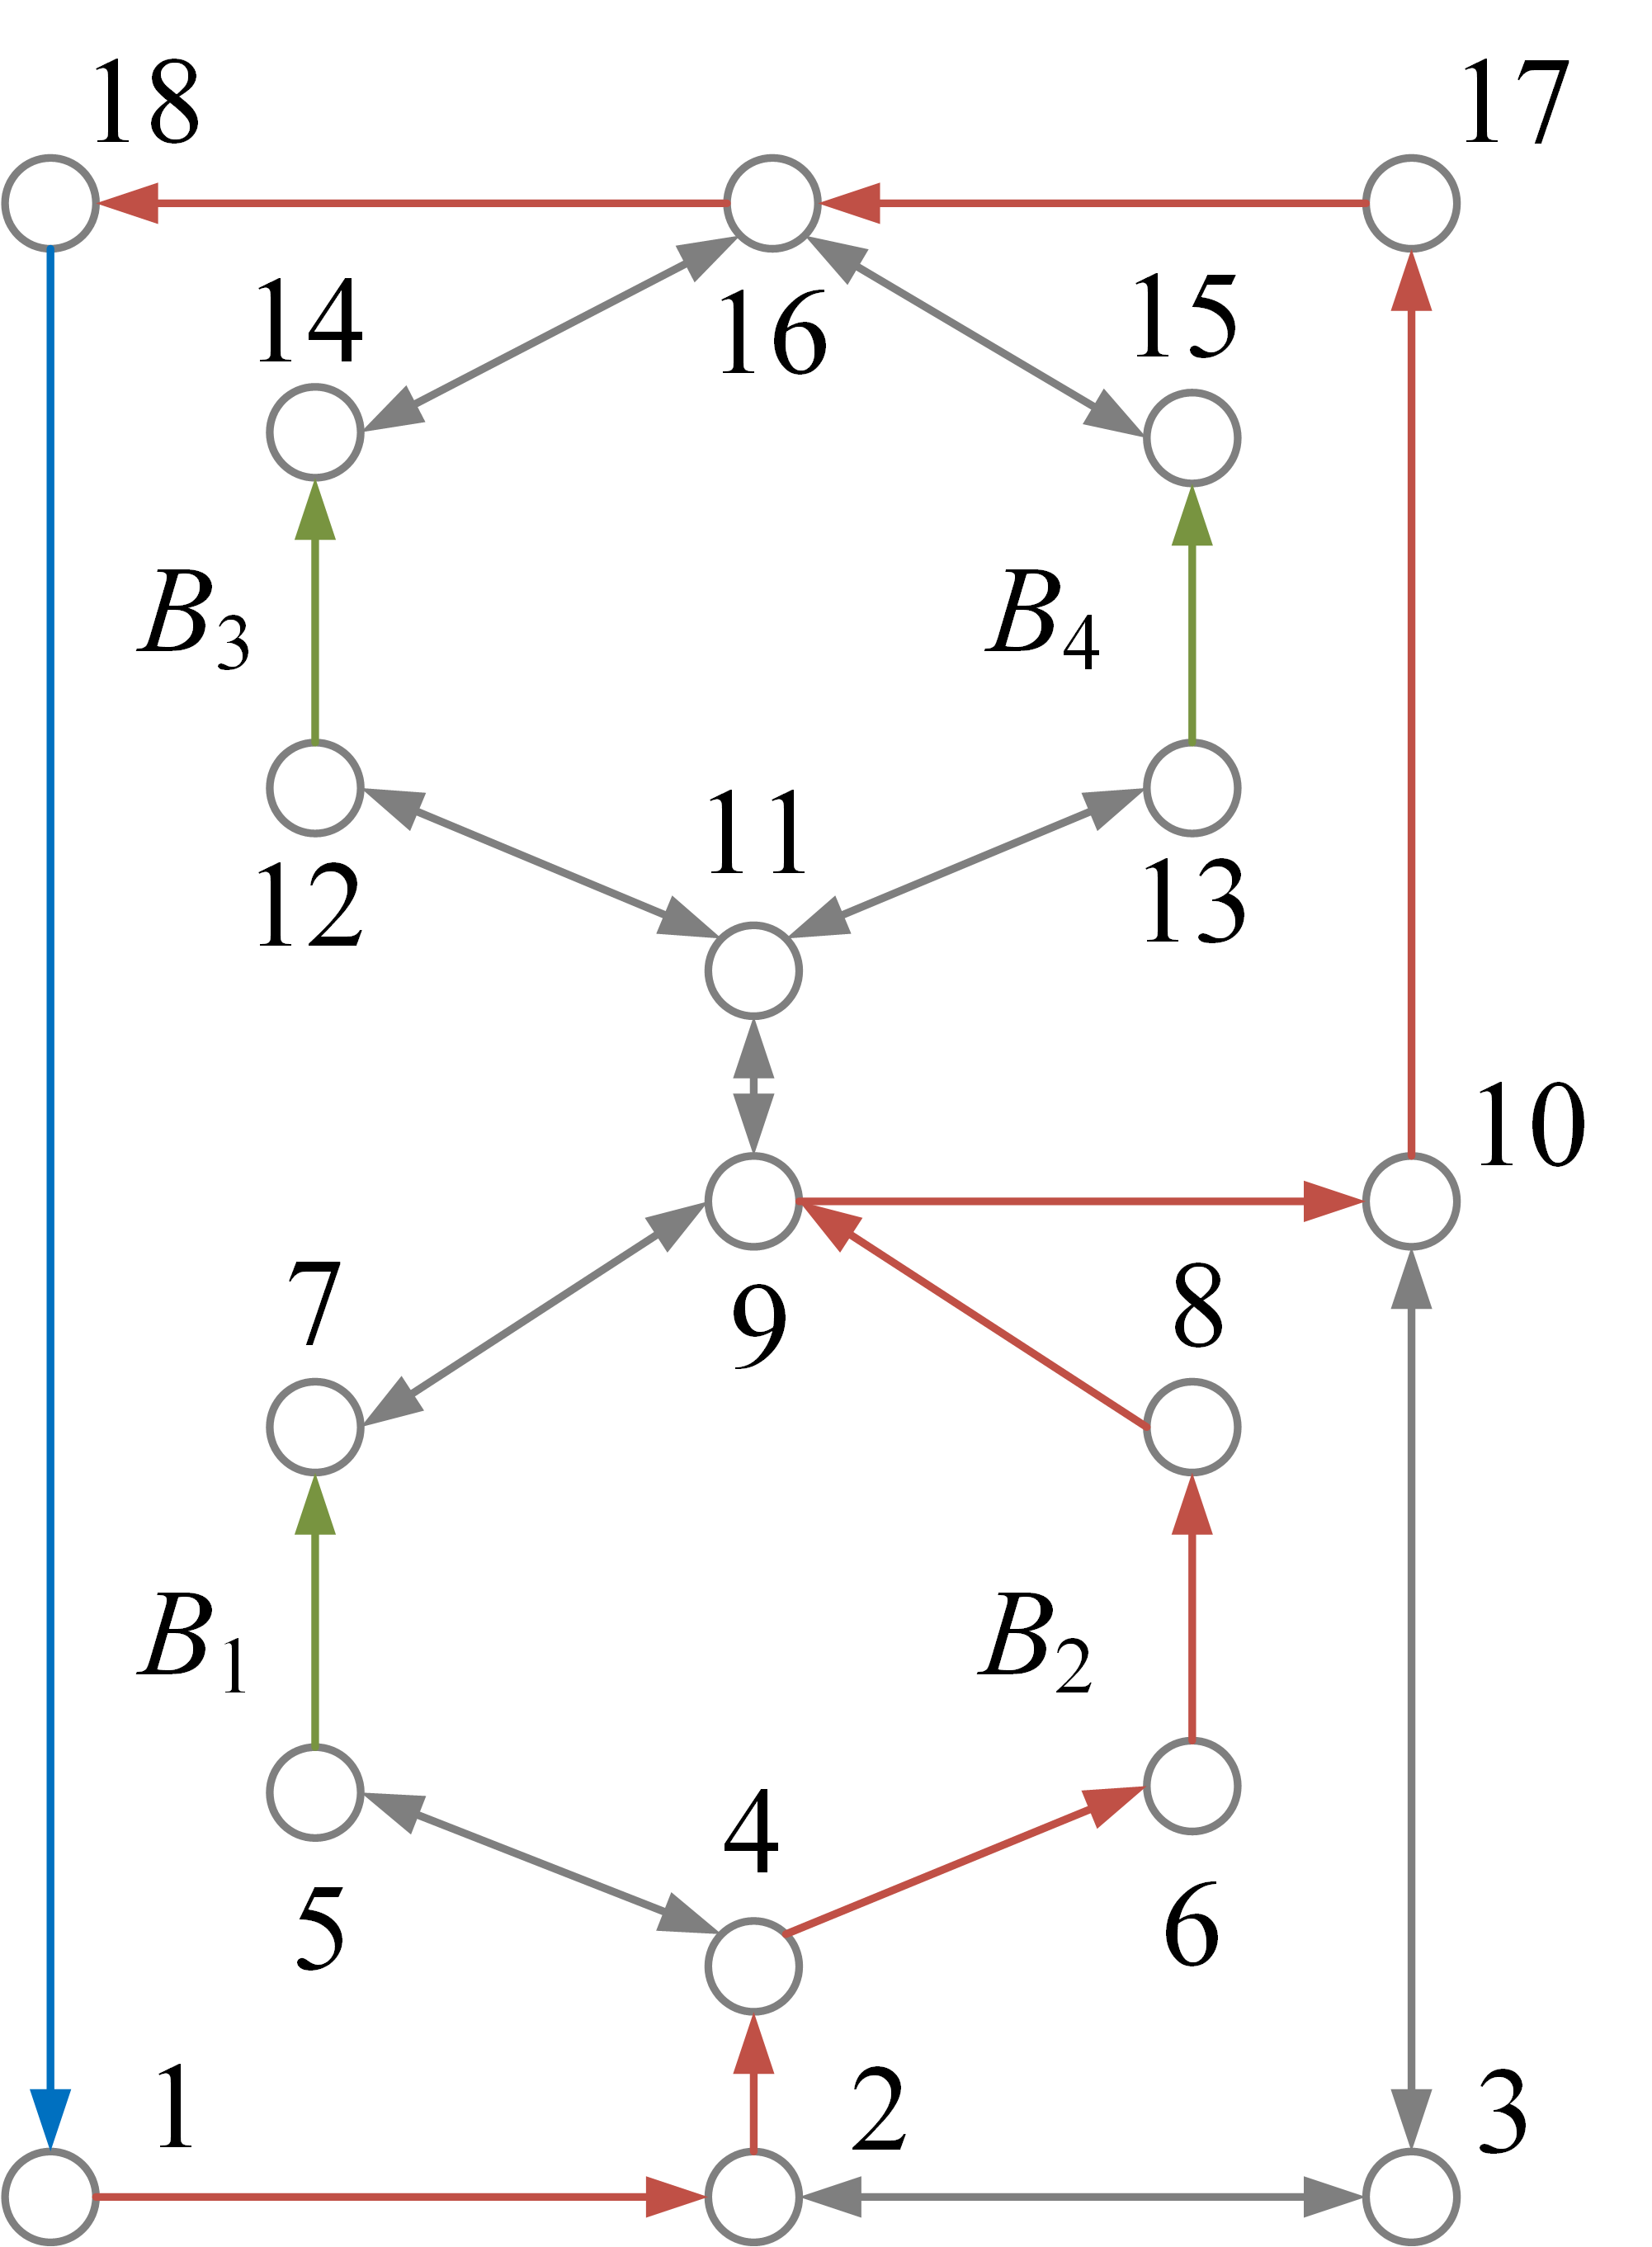
\includegraphics[width=\textwidth]{../attachments/ef-sp2.png}
        \caption{}
        \label{fig:sp2}
    \end{subfigure}
    \\
    \begin{subfigure}[b]{0.45\textwidth}
        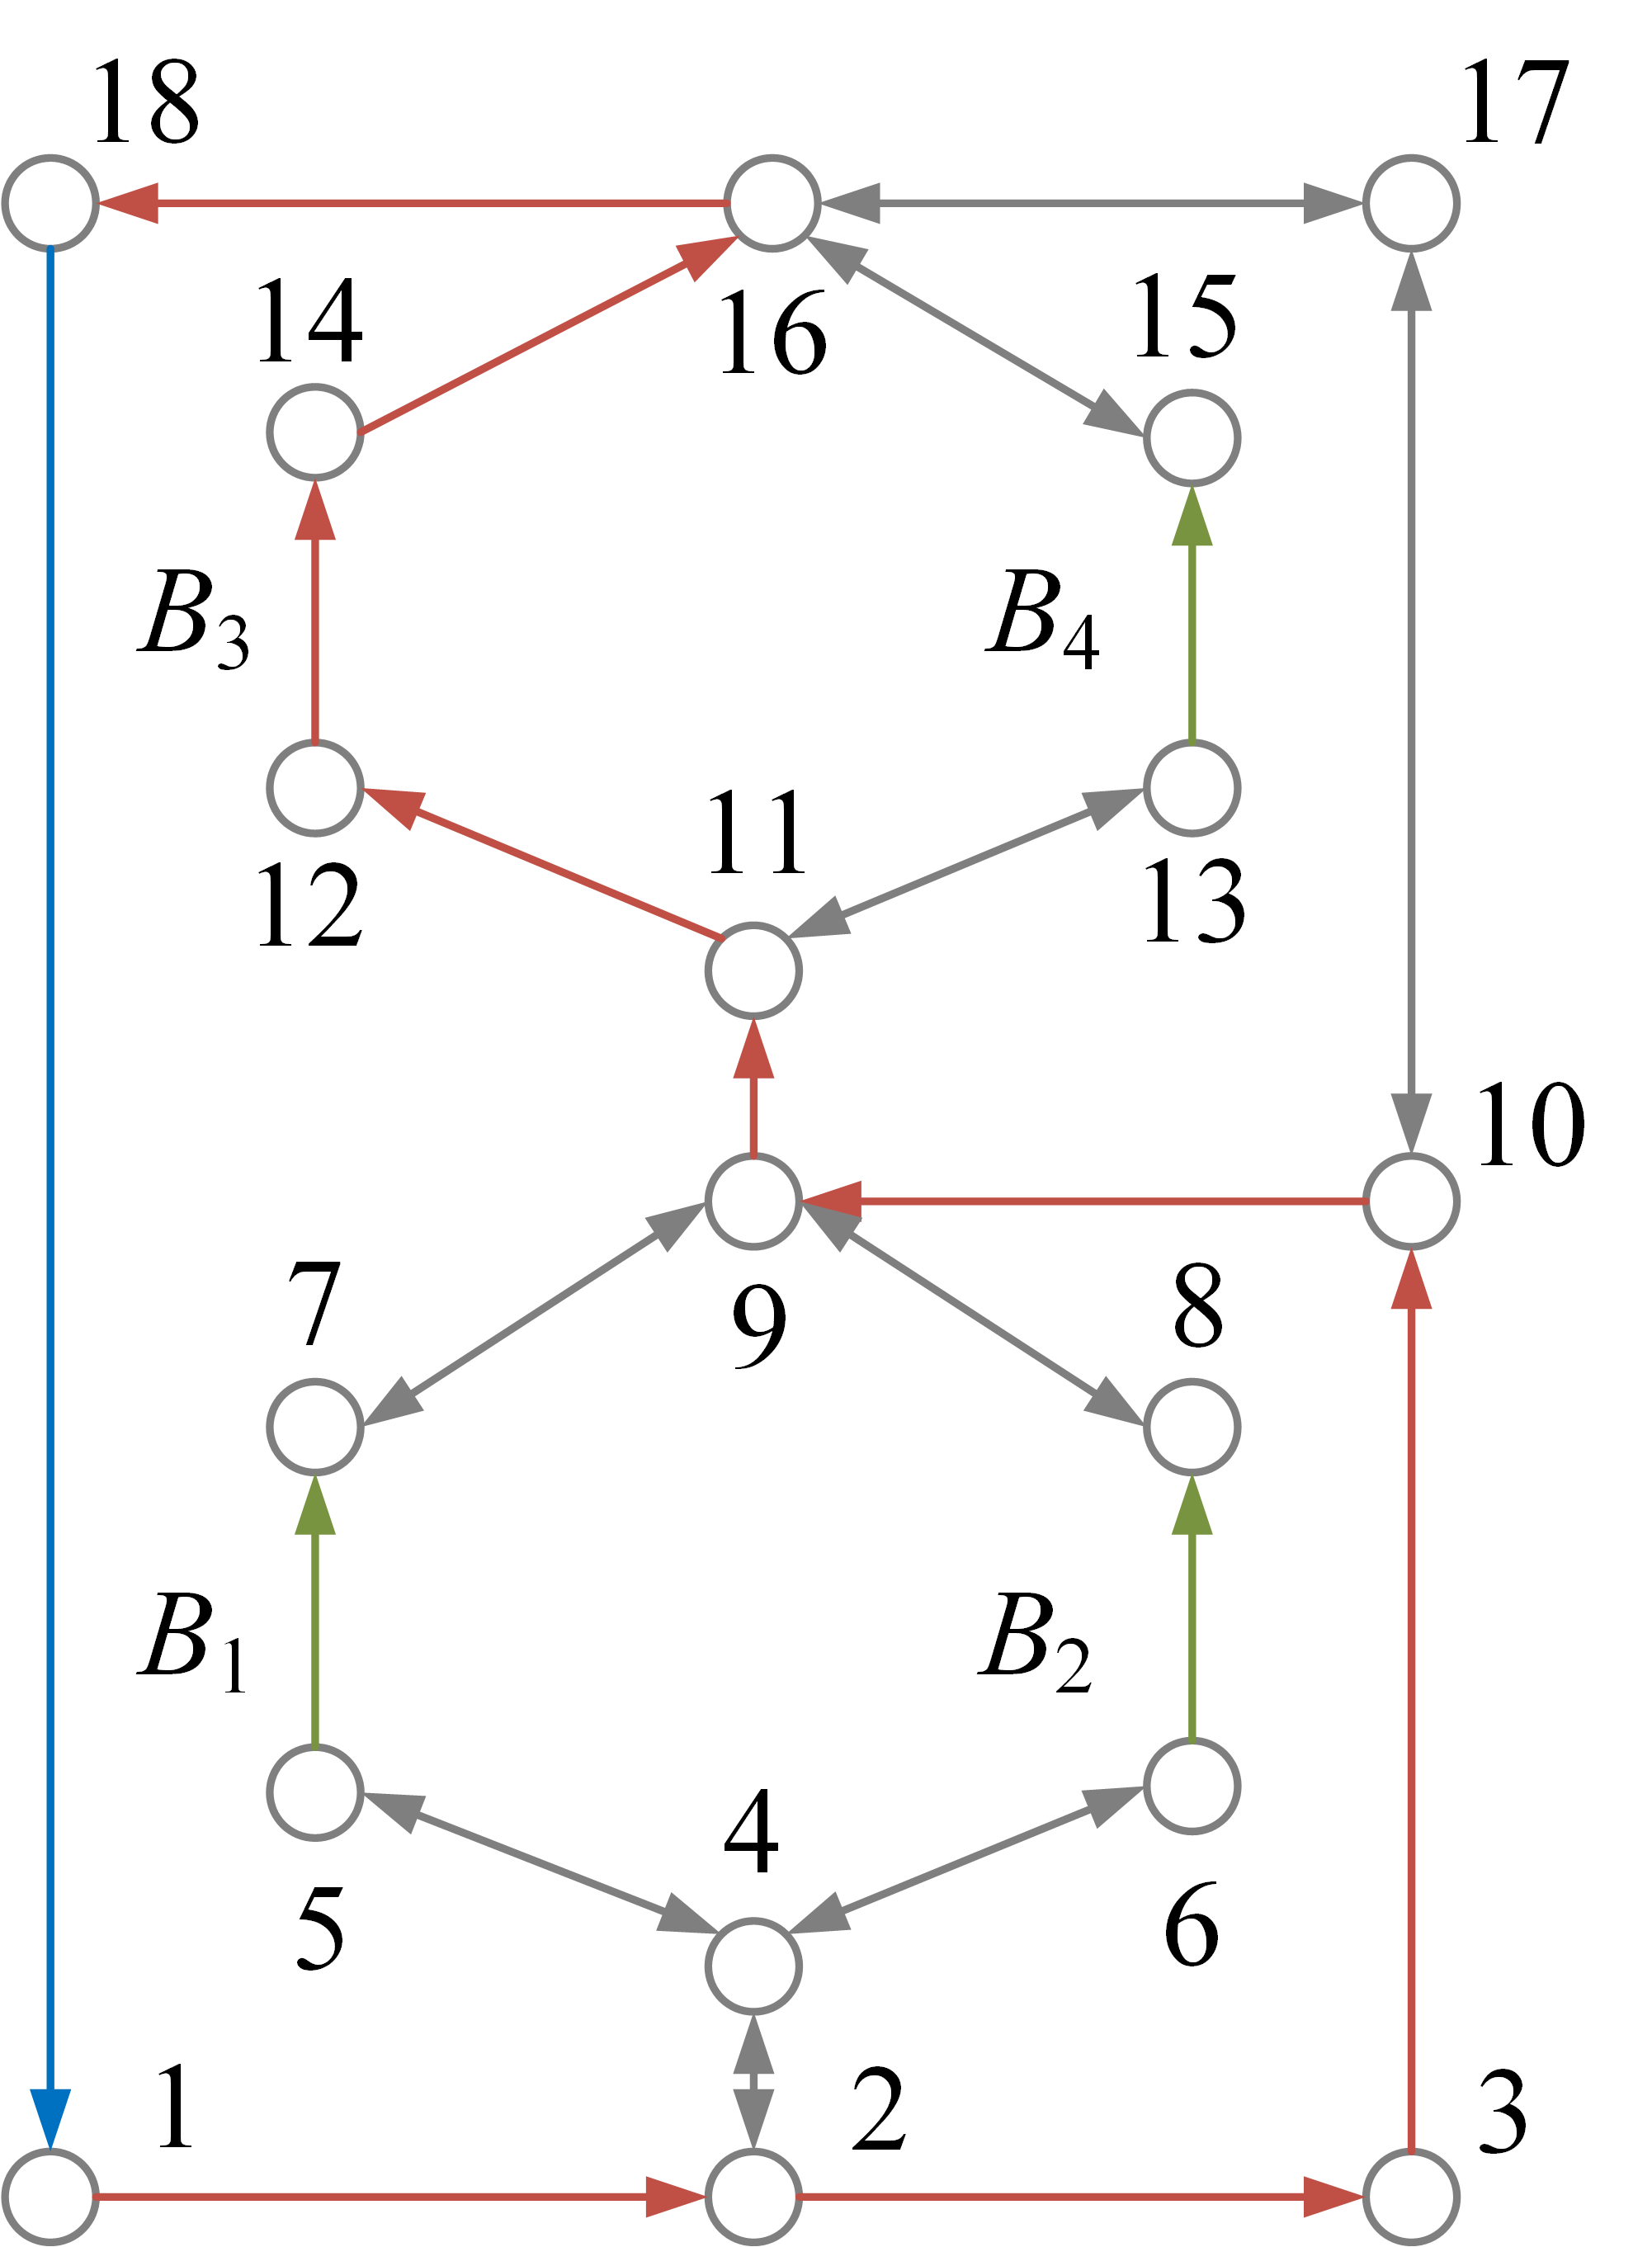
\includegraphics[width=\textwidth]{../attachments/ef-sp3.png}
        \caption{}
        \label{fig:sp3}
    \end{subfigure}
    \hspace{0.05\textwidth}
    \begin{subfigure}[b]{0.45\textwidth}
        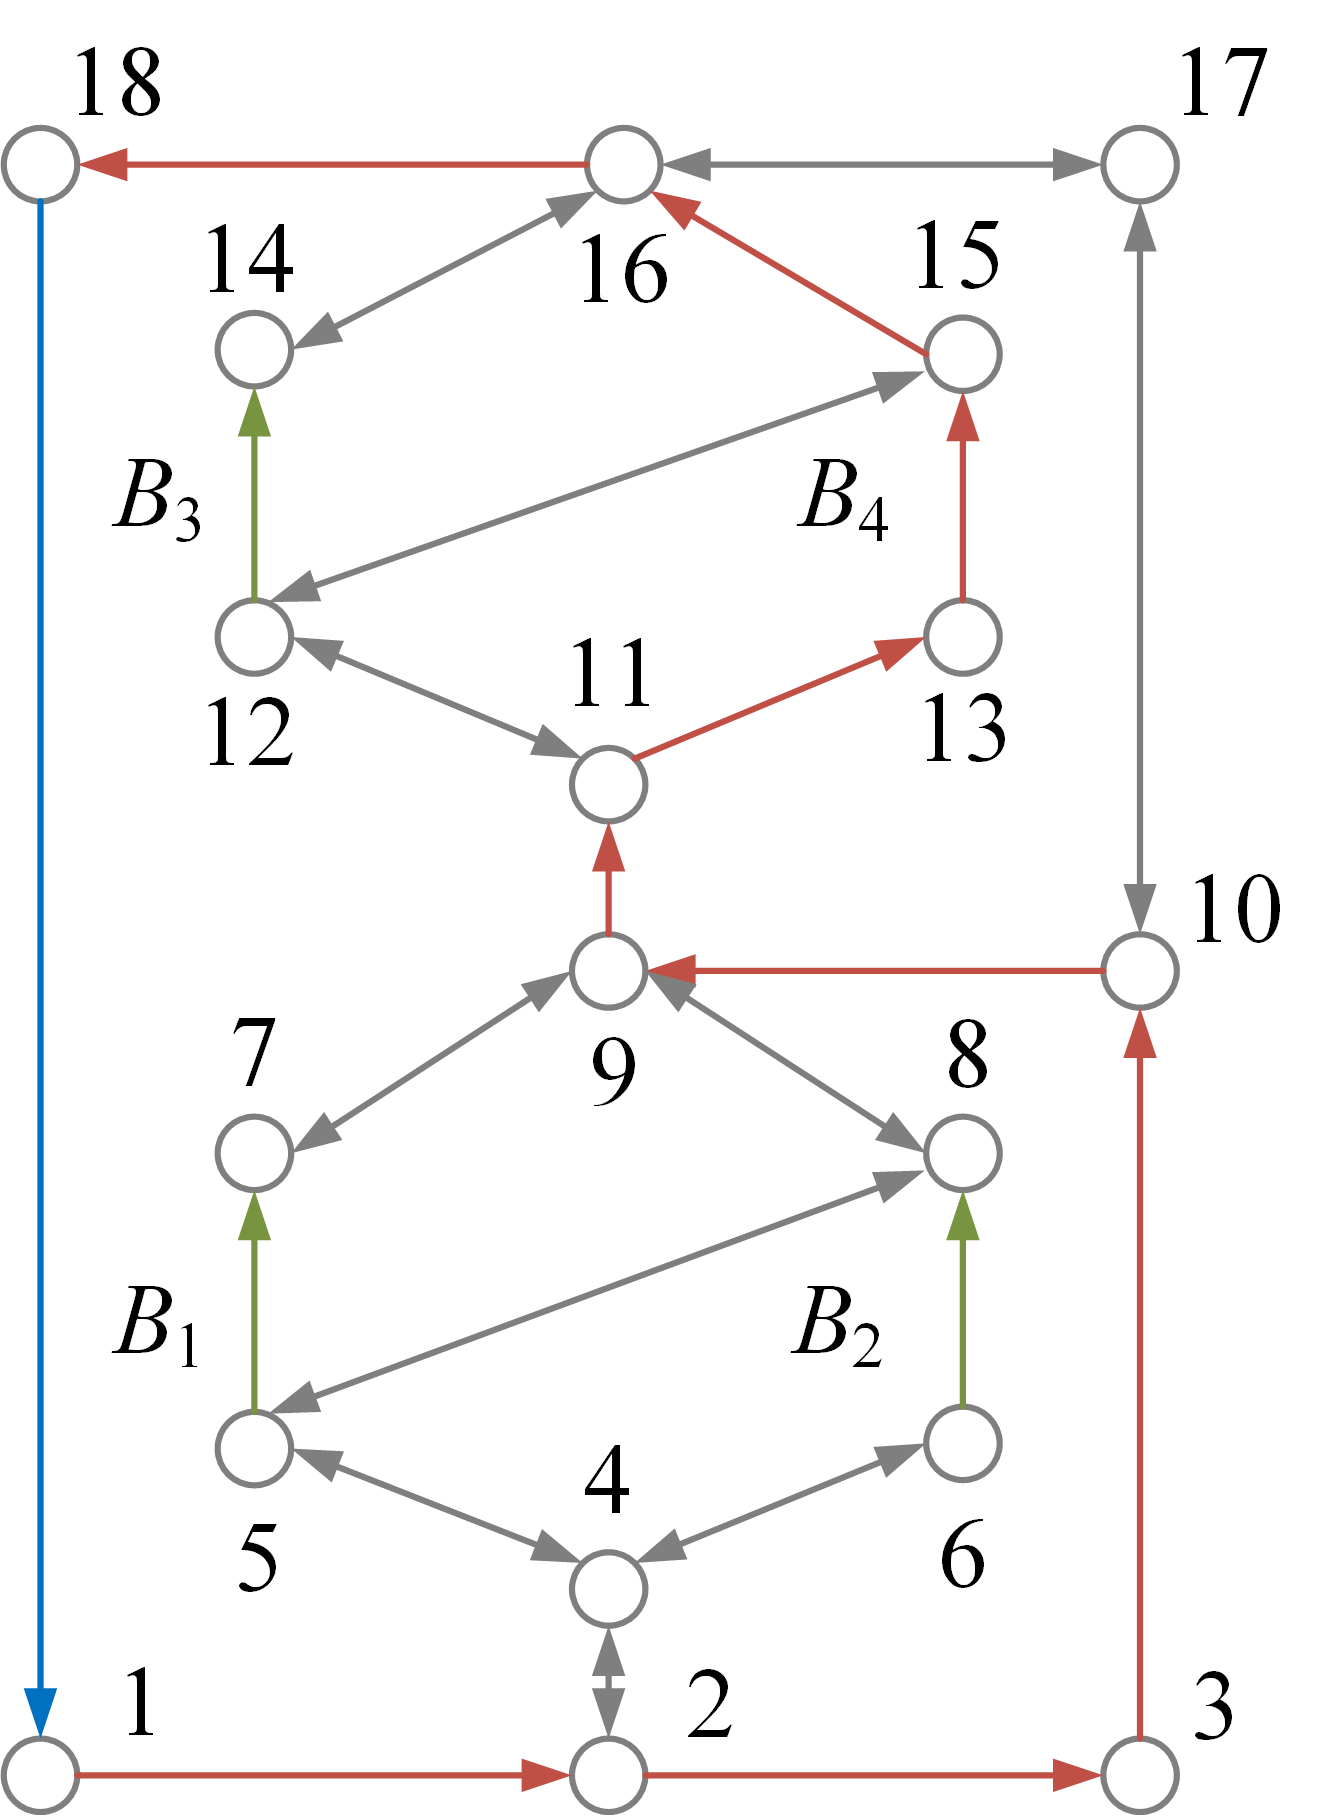
\includegraphics[width=\textwidth]{../attachments/ef-sp4.png}
        \caption{}
        \label{fig:sp4}
    \end{subfigure}
    \caption{
        The $SP$s (highlighted in red) of battery (a)$B_1$ (b)$B_2$ (c)$B_3$ (d)$B_4$ in the complex RBS structure 
        }
\end{figure}

\begin{table}[htbp]
  \centering
    \caption{MAC Calculating result of the output current $I_o$, battery current $\bm{I}_b$ and ratio $\eta$ in the structure combining Lawson et al.\cite{lawsonSoftwareConfigurableBattery2012} and Visairo et al.\cite{visairoReconfigurableBatteryPack2008} with 4 battery cells and 19 switches.} % 修改该caption
    \begin{tabular}{cc}
    \toprule
        % Structure & combining Lawson et al.\cite{lawsonSoftwareConfigurableBattery2012} and Visairo et al.\cite{visairoReconfigurableBatteryPack2008} with 4 battery cells and 19 switches  \\
        Structure & 4 battery cells and 19 switches  \\
    \midrule
    Switch ON & 1,3,5,6,8,9,10,12,18,19 \\
    $\bm{X}_s$ & $\diag(1,0,1,0,1,1,0,1,1,1,0,1,0,0,0,0,0,1,1)$ \\
    \midrule
        $I_o$ & $2u_b/(2R_o+r_b)$ \\
        $\bm{I}_b$ & $[u_b/(2R_o+r_b),u_b/(2R_o+r_b),0,0]$ \\
        $\eta$     & 2 \\
    \bottomrule
    \end{tabular}%
  \label{tab:find_mac}%
\end{table}%

\begin{figure}[htbp]
    \centering
    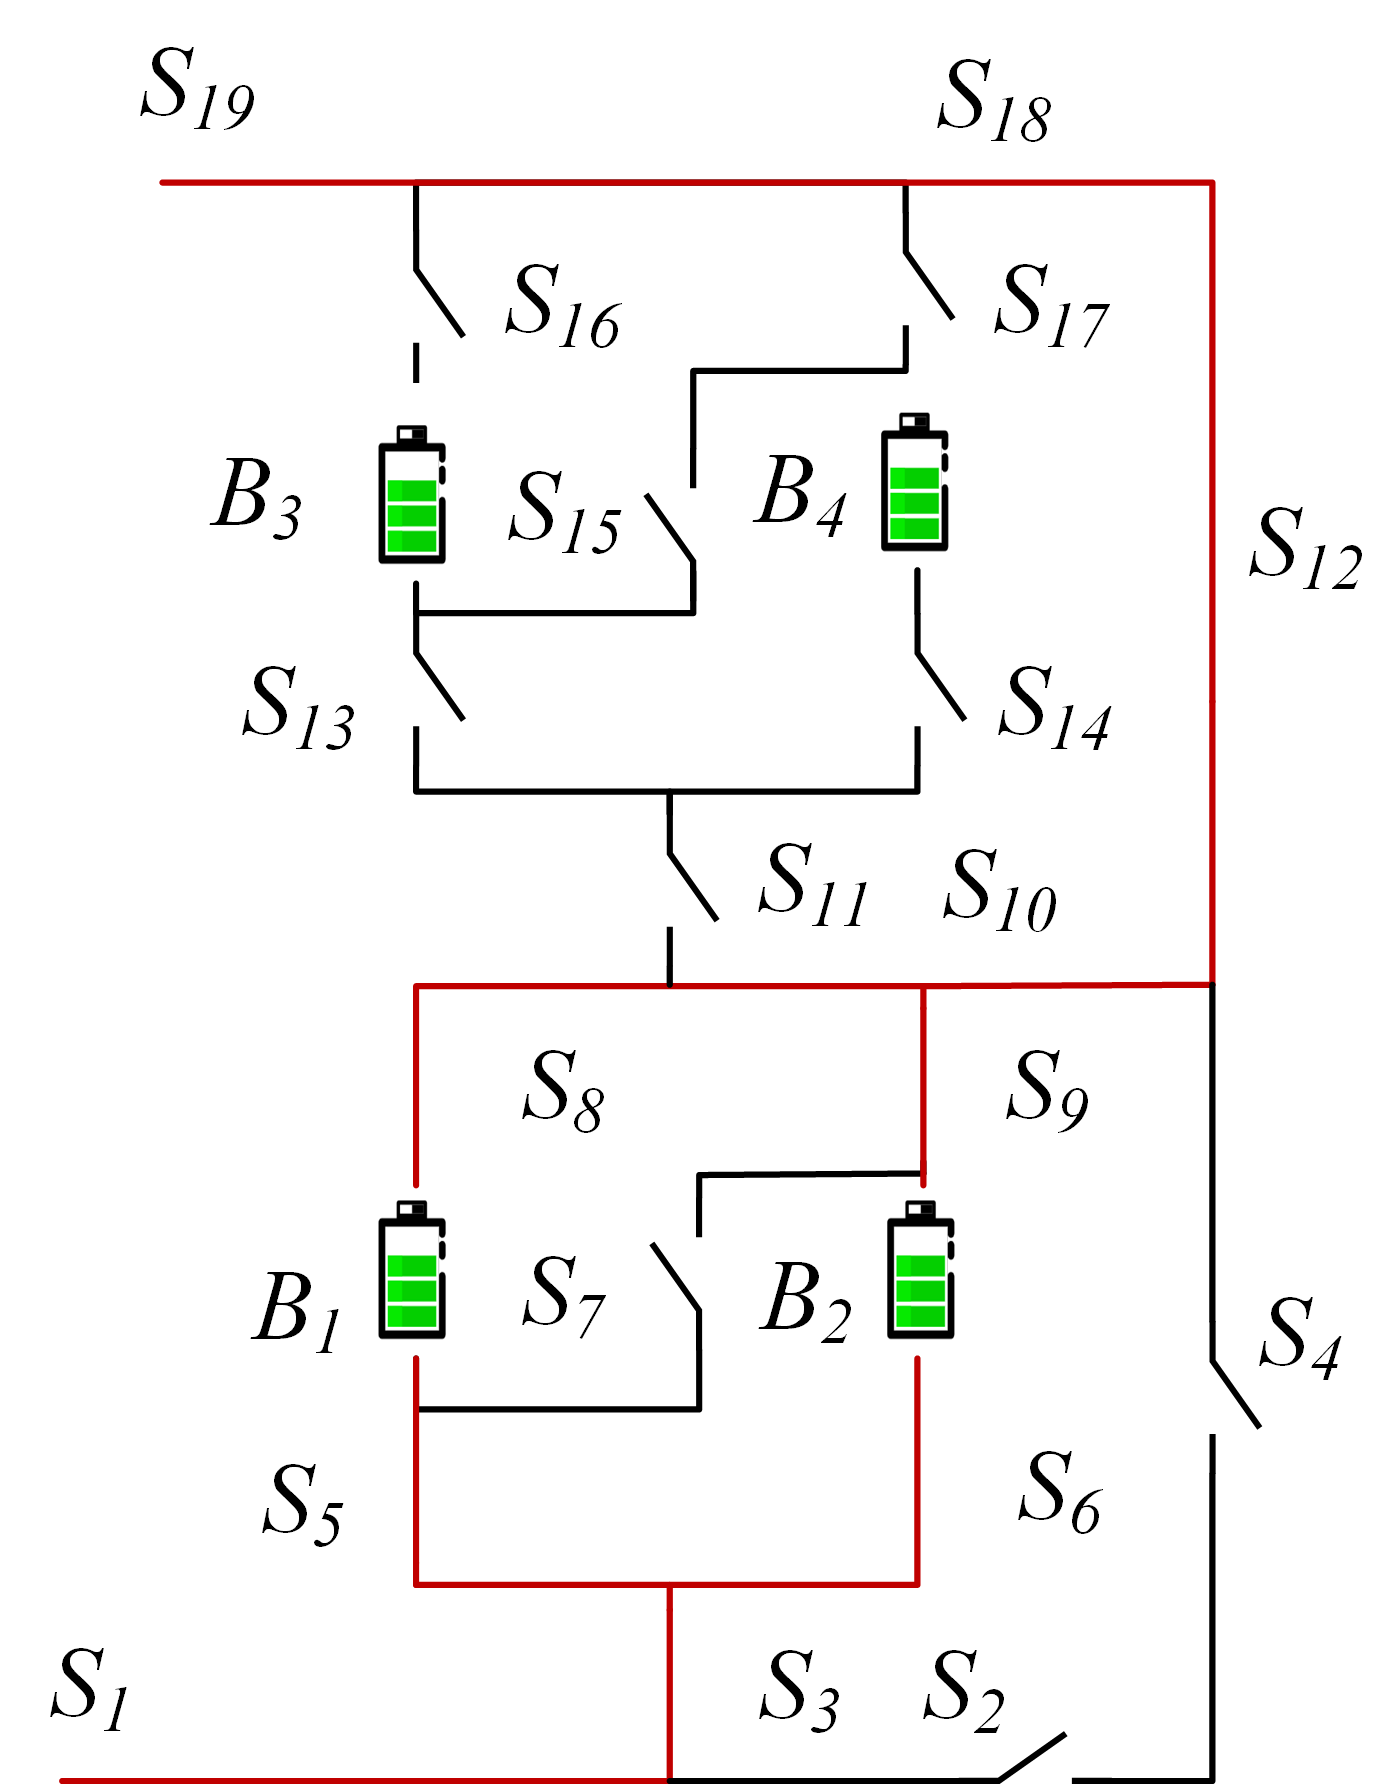
\includegraphics[width=0.5\textwidth]{../attachments/ef-mac.png}
    \caption{
        The finally calculation result of MAC for the new structure with four battery cells and 19 switches.
        The red lines represent the branches through which the current flows, and the switches on these branches are ON. 
        In this situation, the RBS outputs MAC to the outside, which is $\eta=2$.
    }\label{fig:ef-mac}
\end{figure}

\subsection{Discussion}

First, the correctness of the results in Fig. ref{fig:ef-mac} is discussed here.
When $B_1$ and $B_2$ or $B_3$ and $B_4$ are connected in parallel, the RBS can output the maximum current, which is $\eta=2$, i.e. twice the current output of a single battery in RBS.
While adding more batteries to the main circuit can only form a series structure and will not improve the MAC.
It is worth noting that when solving for MAC, $\eta$ is used as the objective function instead of $I_o$, which makes the result of MAC more reasonable. 
According to the results shown in Tab. \ref{tab:find_mac}, $I_o$ and $\bm{I}_b$ are affected by the equivalent resistance $R_o$ of external electrical appliance, the battery's electromotive force $u_b$, and internal resistance $r_b$. % Io 和 Ib 是 xxx的函数
This means that if $I_o$ is used as the objective function, even for the same RBS structure, the MAC result and corresponding switch state could be changed due to different external electrical appliances. 
This increases the difficulty and uncertainty in RBS structure design. 
On the contrary, by using $\eta$ as the objective function, which dividing $I_o$ and $\max\bm{I}_b$, the influence of these factors on the results is eliminated, as shown in Tabs. \ref{tab:given_x} and \ref{tab:find_mac}.
$\eta$ only reflects the maximum output current capability of the RBS structure.
Assuming that the maximum allowed current of battery cells in the RBS is $I_m$, the maximum output current of the RBS structure can be calculated as $\eta I_m$ by calculating the $\eta$ of the structure. 
Therefore, compared to $I_o$, $\eta$ is more suitable for structure design. 
Most of the currently proposed RBS structures\cite{ciNovelDesignAdaptive2007,alahmadBatterySwitchArray2008,kimDependableEfficientScalable2010b,kimBalancedReconfigurationStorage2011a,taesickimSeriesconnectedSelfreconfigurableMulticell2012a,6843711} have simple topological characteristics, and the calculation of MACs are relatively simple, even intuitive. % #TODO 添加cite
However, when complex and flexible structures need to be designed for application scenarios such as equalization or isolation of specific battery cells, the estimation of MAC will become complex and complicated. 
The method proposed in this paper can effectively solve any RBS structure and estimate MAC universally, paving the way for the structure design of more complex and flexible RBSs.


When the RBS has isolated battery cells, the original topology of the structure is altered. 
However, the method proposed in this paper can still be used to calculate the MAC of the new structure. 
The MAC after the isolation operation can be obtained by calculating the new structure following the procedures described in the previous subsection.
During the calculation process, the isolated battery cell(s) do not participate in the calculation, i.e., their nodes, edges, and $SP$s are not considered. 
The MACs under various isolated battery cell(s) are calculated on the structures proposed by Lawson et al. (Fig. \ref{fig:arch-e}), Visairo et al. (Fig. \ref{fig:arch-f}), and the new structure that integrates the previous two structures (Fig. \ref{fig:ef-topo}), as shown in Fig. \ref{fig:isolated_mac}. 
For the structure proposed by Lawson et al., the MAC remains the same as that without isolated battery cells, i.e., $\eta=1$, when the number of isolated battery cells increases, until all the cells in the RBS are isolated.
For the structure proposed by Visairo et al., the MAC decreases as the number of isolated battery cells increases, until $\eta=0$.
While the new structure has two cases of isolating two cells, one is to isolate two cells within the same substructure, in which case $\eta=2$; the other is to isolate one cell in each of the two substructures, in which case $\eta=1$. 
Overall, the MAC of the new structure is positioned between the structures proposed by Lawson et al. and Visairo et al..
It can be seen that the MAC of the structure in Fig. \ref{fig:arch-e} is the most stable, and the structure has advantages in isolation and redundancy backup, but its MAC is the smallest. 
The structure proposed shown by Fig. \ref{fig:arch-f} can output the largest MAC but is susceptible to the number of isolated battery cells. 
However, the structure proposed by this paper has certain advantages in both aspects, being insensitive to the number of isolated battery cells while simultaneously achieving a larger MAC.

\begin{figure}[htbp]
    \centering
    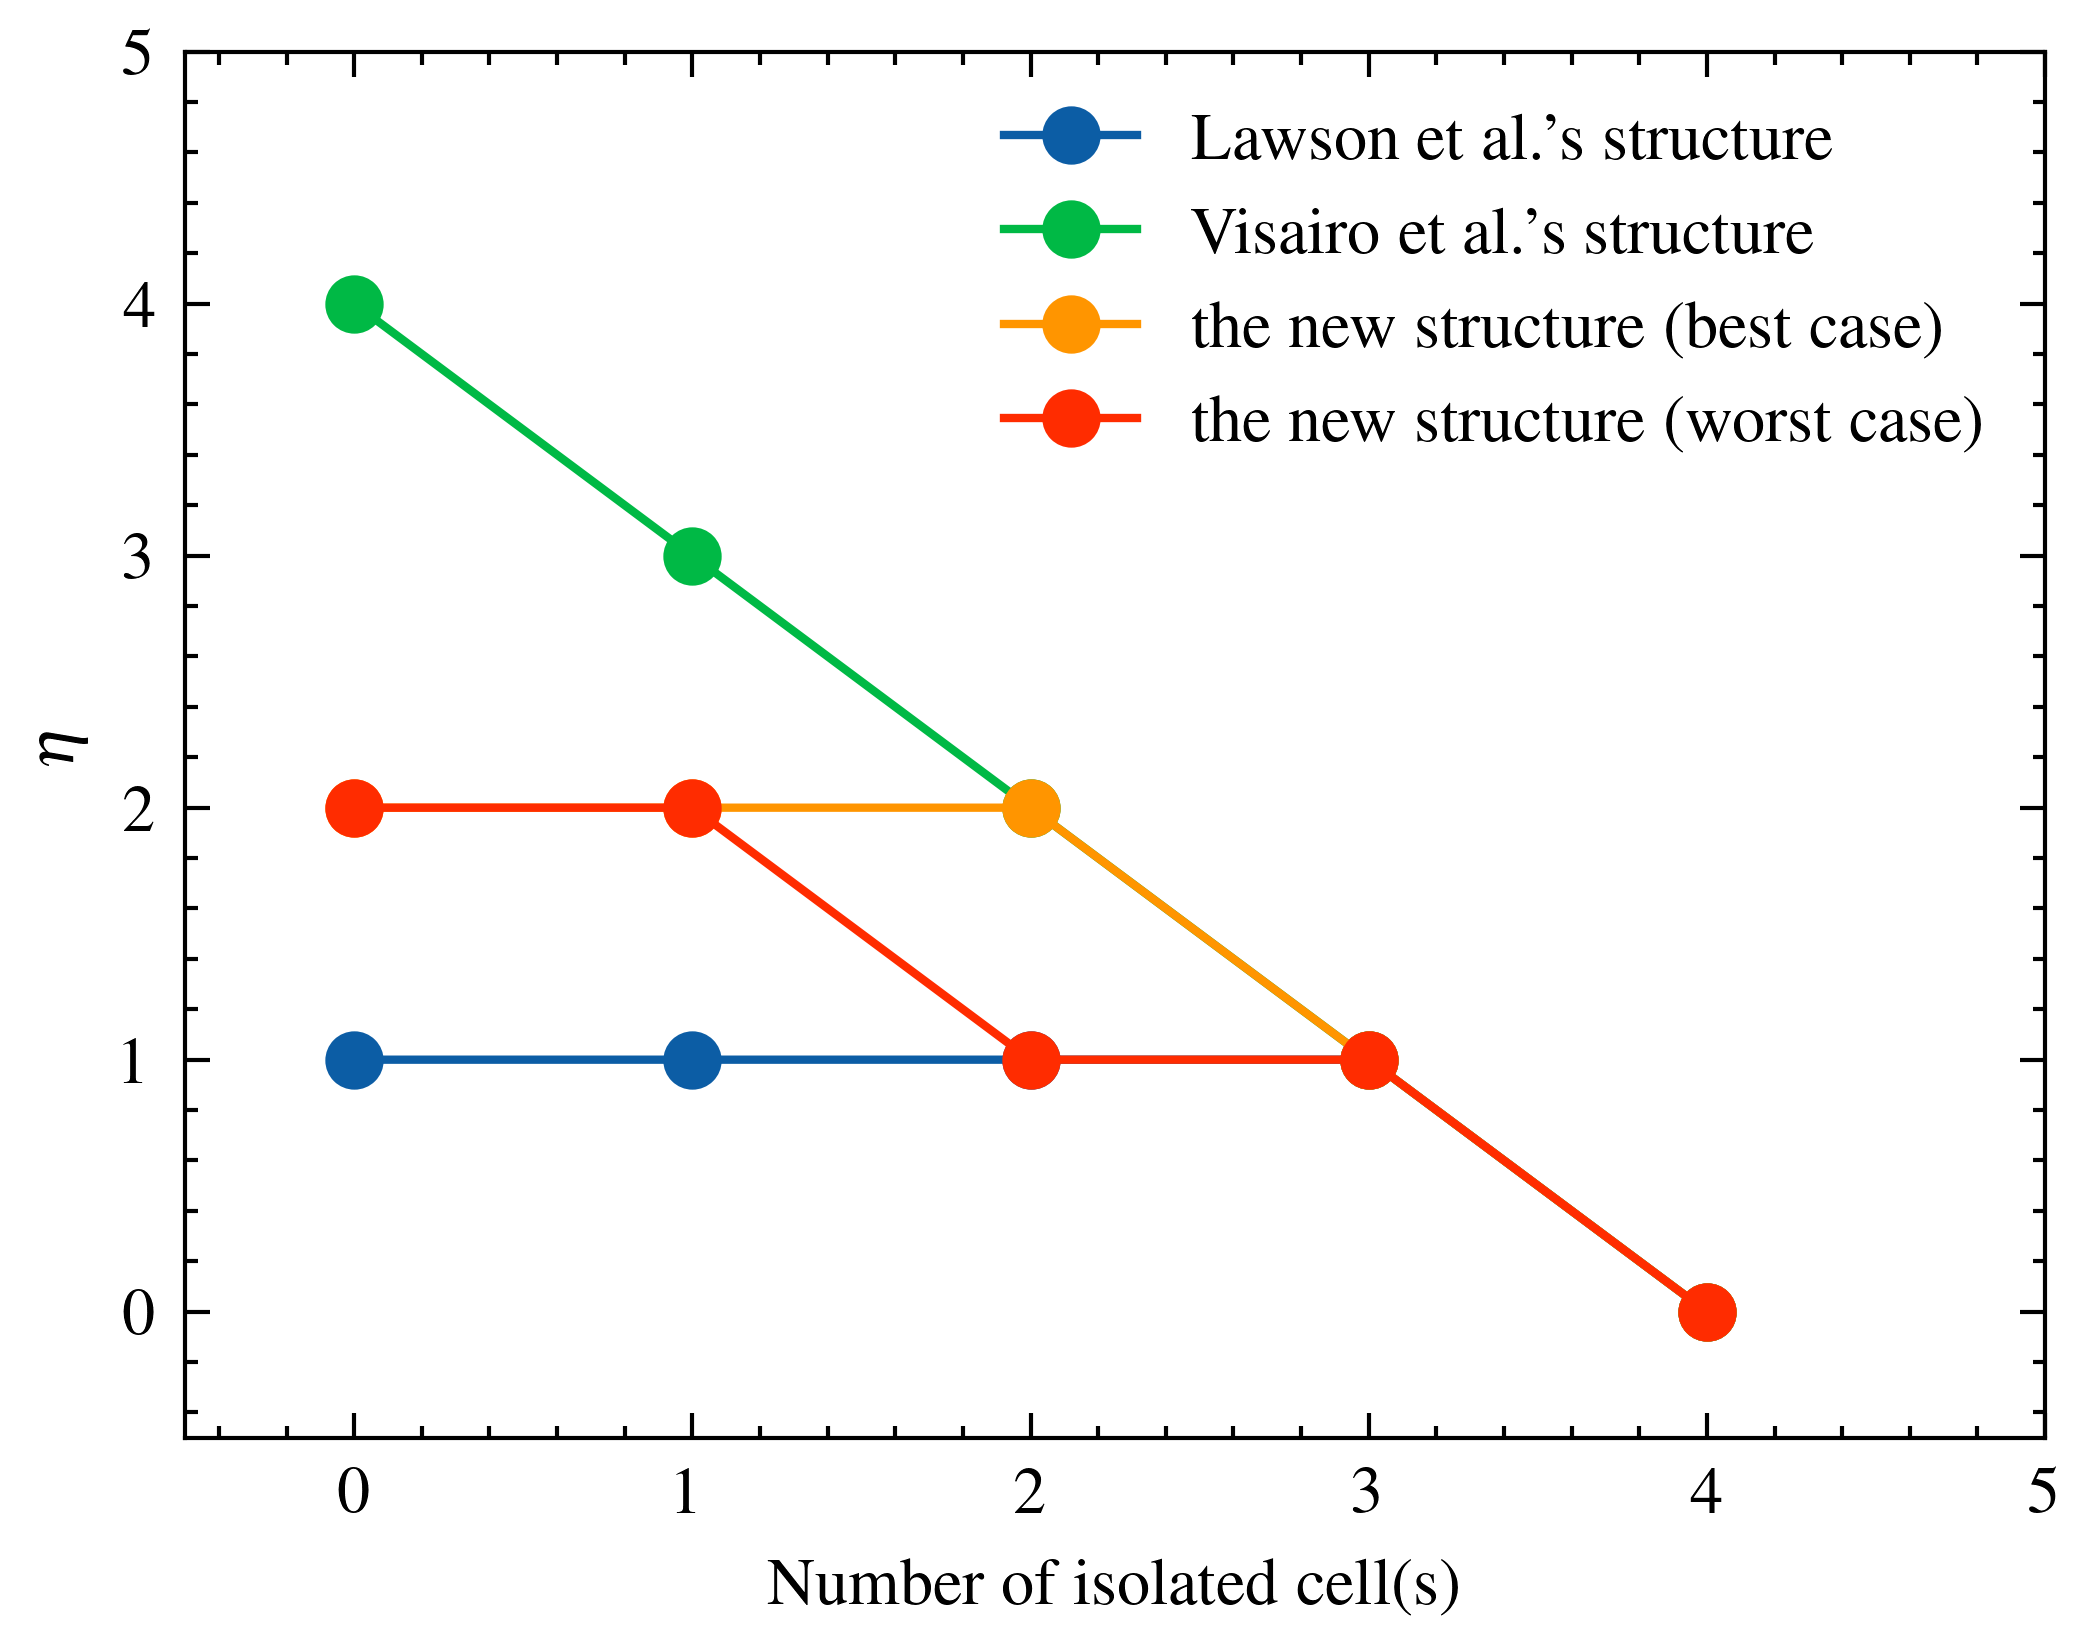
\includegraphics[width=0.8\textwidth]{../attachments/isolated_mac.png}
    \caption{
        The variation of MAC with the number of isolated battery cells for different RBS structures, including the structure proposed by Lawson et al., Visairo et al. , and the new structure in this paper.
    }\label{fig:isolated_mac}
\end{figure}

\section{Conclusion}

This paper firstly proposes a method to calculation the MAC of RBS according to its architecture. 
To find the circuit in RBS that enable the MAC, a greedy strategy incorporate with the topologic model is developed to. 
The effectiveness of proposed method is tested on a more complex RBS structure based on two proposed structure.
This work presents an effective approach to evaluate the MAC of RBS, which is essential for design and management of the RBS. 
Future research could focus on developing new performance indicators for evaluating RBS performance using the currents and voltages obtained by this method, as well as modifying the equivalent model of the battery to enable more accurate simulations of RBS, including transient analysis.

\section{Appendix} 
\begin{algorithm}% #TODO 待修改
    \caption{Get the max available currents of a certain RBS}\label{alg:eta_RBS}
    \KwData{Directed graph model $G(V,E)$ of the RBS}
    \KwResult{$\max \eta$}
    \For{$i \in E_b$}{
        $P_i \leftarrow \{path| \text{starts at $v_1$ and ends at $v_n$} \}$\;
        $SP_i \leftarrow p_i \text{ which has the minimum}~\omega(p_i)~\text{among all}~p_i \in P_i. $
    }
    get $\bm{A}$ by Equation \ref{eq:A}\;
    \While{not yet determine $\max \eta$ }
    {
        $N_{sel} \leftarrow \text{number of selected $SP$s calculated by dichotomy}$\;
        $C_b    \leftarrow \text{set of all combinations of $N_{sel} $~batteries from $N_b$}$\;
        \For{$c_b \in C_b$}{
            $\bm{x}_s \leftarrow \text{list of all switches' state: $x_s[j]=1$ if $ j \in \bigcup_{i\in c_b}SP_i $ else 0}$\;
            $\bm{X} \leftarrow diag[1,1,\cdots,1,\bm{x}_s] $\;
            get $\bm{Y}_n$ by Equation \ref{eq:Yn}\;
            \eIf{$\bm{Y}_n$ is invertible}{
            }{construct an effective solution}
            get $I_o$ by Equation \ref{eq:I_o}\;
            get $\bm{I}_b$ by Equation \ref{eq:I_b}\;
            \eIf{$\max(\bm{I}_b)\leq I_m$}{
                $\eta \leftarrow I_o/\max(\bm{I}_b)$\;
            }{break}
        }
    }
\end{algorithm}

\section{Acknowledgement}
This work was supported by the National Natural Science Foundation of China (NSFC, No.52075028).

\bibliographystyle{ieeetr}
\bibliography{my_ref}

\end{document}
